\documentclass[aspectratio=169, 12pt]{beamer}
% Note: You can use the handout mode by changing to [aspectratio=169, 12pt, handout]. This results in the pauses being removed.

\newcommand{\handout}{false}
% This command excludes certain frames when the boolean is set to true.

\usepackage{algorithm}
\usepackage{algpseudocode}
\usepackage{amsmath}
\usepackage{amsthm}
\usepackage{blindtext}	% TODO Remove
\usepackage{changes}
\usepackage[nameinlink,capitalise]{cleveref}
\usepackage{enumitem}
\usepackage{amsbsy}
\usepackage{afterpage}
\usepackage{hyperref}
\usepackage[acronym]{glossaries} % toc does not work properly
\usepackage{siunitx}
\usepackage{subcaption} 
\usepackage{thmtools}
\usepackage{tikz}

\usetikzlibrary{automata,arrows,shapes}

\makeglossaries

\graphicspath{{./figures/}}

%% Glossary and Acronyms %%
%% List of acronyms %%
% Reference definition:
% - \newacronym[options]{label}{short}{long}
%	options: description, longplural, ...
%
% Reference usage:
% - \acrlong{label}  : displays the full text of the acronym
% - \acrshort{label} : displays the abbreviation
% - \acrfull{label}  : displays the full text followed by the abbreviation
% - \acrshortpl{label} : the plural of the abbreviation (similarly for acrlongpl and acrfullpl)

\newacronym{acr:dtp}{DTP}{Decision-Theoretic Planning}

\newacronym{acr:hmm}{HMM}{Hidden Markov Model}

\newacronym[longplural=Markov Decision Processes]{acr:mdp}{MDP}{Markov Decision Process}

\newacronym{acr:pomdp}{POMDP}{Partially Observable \acrshort{acr:mdp}}

\newacronym{acr:sdm}{SDM}{Sequential Decision Making}
%% Glossary Entries:
%
% Reference definition:
% \newglossaryentry{maths}
% {
% 	name=mathematics,
% 	description={Mathematics is what mathematicians do}
% }
%
% Reference usage:
% - \gls{ } Prints term lower case
% - \Gls{ } Prints term upper case
% - \glspl{ } Prints term plural lower case
% - \Glspl{ } Prints term plural upper case

\newglossaryentry{maths}{
	name={mathematics},
	description={Mathematics}
}

\newcommand\mat[1]{\pmb{#1}}
\newcommand\arr[1]{\pmb{#1}}
\DeclareMathOperator*{\argmax}{arg\,max}

%% Custom Definitions %%
\def\subsubsectionautorefname{Section}
\def\subsectionautorefname{Section}
\def\sectionautorefname{Section}
\def\chapterautorefname{Chapter}
\def\algorithmautorefname{Algorithm}

%\declaretheoremstyle[bodyfont=\normalfont]{normalbody}
%\declaretheorem[style=normalbody,name=Definition]{definition}
\theoremstyle{definition}
\newtheorem{definition}{Definition}
\newtheorem*{problem}{Problem Statement}

%% Pseudocode settings %%
\newcommand*\Let[2]{\State #1 $\gets$ #2}
\algrenewcommand{\algorithmiccomment}[1]{\hfill$\rhd$ #1} % Fix for comments in pseudocode

%% Title and Cover Pages %%

%% Use Roman numerals for the page numbers of the title pages and table of
%% contents.
\frontmatter

%% Uncomment following 16 lines for a cover with a picture on the lower half only
\title[tudelft-white]{Learning and Optimizing Probabilistic Models for Planning Under Uncertainty} %in Mobile Robot Navigation}
%\subtitle[tudelft-black]{Optional subtitle}
\author[tudelft-white]{R. van Bekkum}
\affiliation{Delft University of Technology}
\coverimage{figures/tank.jpg}
\covertext[tudelft-white]{
	\textbf{Cover Text} \\
	possibly \\
	spanning 
	multiple 
	lines
	\vfill
	ISBN 000-00-0000-000-0
}
\setpagecolor{tudelft-cyan}
%\makecover[split]

% TEMPORARY
\newcommand{\showoutline}[1]{
	\vspace{0.3cm}
	\hrule
	\vspace{0.3cm}
	{\large\textbf{PLANNED OUTLINE}:}
	\vspace{0.3cm}
	\hrule
	\vspace{0.3cm}
	{#1}
	\vspace{0.3cm}
	\hrule
	\vspace{0.3cm}	
}

%\title{Learning Probabilistic Models for Planning under Uncertainty by Bayesian Optimization of Unsupervised Machine Learning Algorithms for State-Spaces\vspace{8 pt}
\title{Learning and Optimizing Probabilistic Models for Planning under Uncertainty in Mobile Robot Navigation\vspace{18pt}
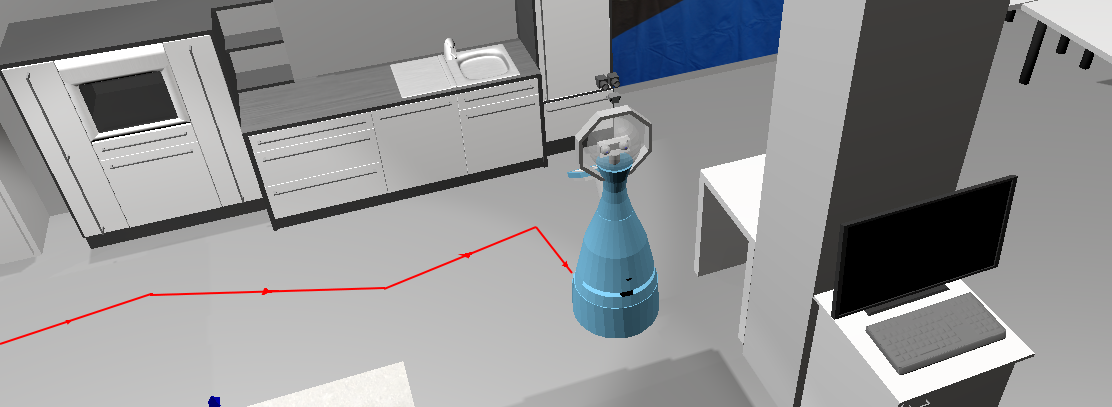
\includegraphics[width=0.5\textwidth]{figures/simulator_3}\vspace{-18pt}}
%\subtitle{\textcolor{darkerblue}{}}

%\titlegraphic{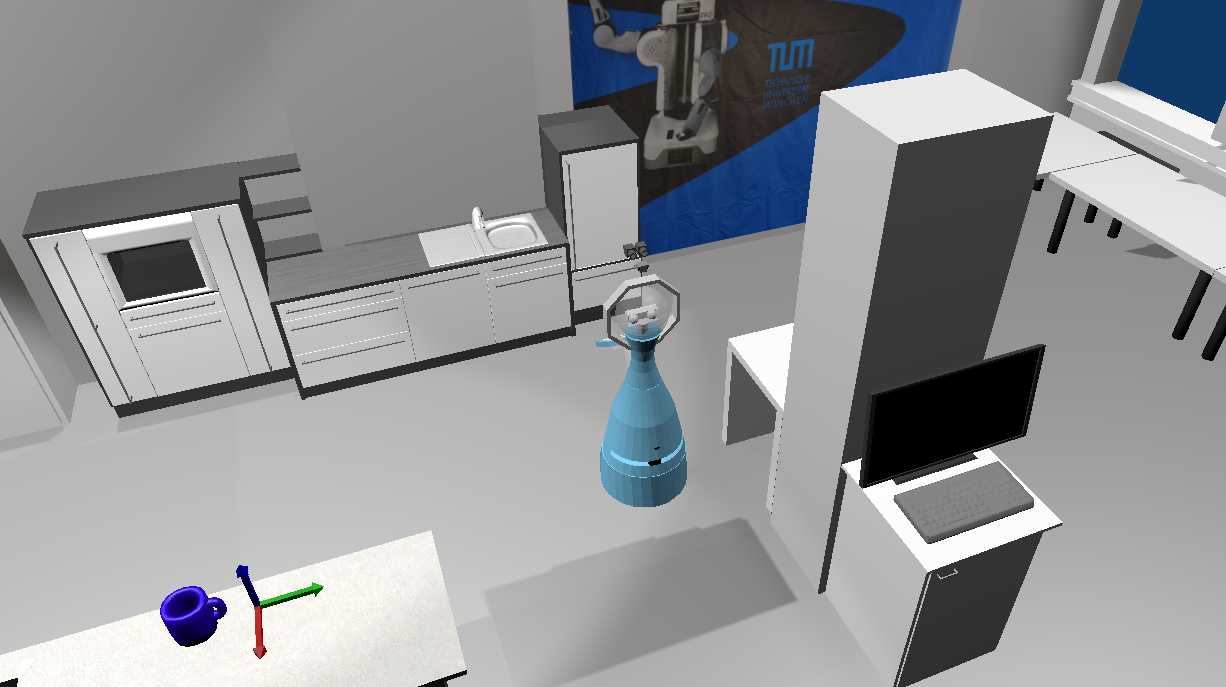
\includegraphics[width=\textwidth,height=.5\textheight]{figures/simulator}}

\author{\vspace{-7pt}Rob van Bekkum}
\institute{\vspace{-7pt}Delft University of Technology}

\date{April 5, 2017}

\begin{document}

\begingroup
\setbeamertemplate{headline}{%
	\leavevmode%
	\hbox{%
		\begin{beamercolorbox}[wd=\paperwidth,ht=2.5ex,dp=1.25ex]{palette tertiary}%
		\end{beamercolorbox}%
	}
}

% Title Sheet
\frame{\titlepage}

\endgroup

\section{Decision-Theoretic Planning}

\begin{frame}
\frametitle{Decision-Theoretic Planning}
\framesubtitle{DTP Problem Scope}

\begin{columns}[T]
 	\begin{column}{.7\textwidth}
	\textbf{Systems:}
	\begin{itemize}
		\item Dynamics are stochastic, i.e., involve uncertainty
		\begin{itemize}
			\item Execution of actions (e.g., robot may slip)
			\item Exogenous events (e.g., doors open/closed)
			\item Observations (e.g., sensor noise)
		\end{itemize}
		\item Controlled by one or more agents
		\item Sequential decisions of actions to execute
	\end{itemize}
%	\textbf{Examples:}
%	\begin{itemize}
%		\item Motion Planning
%		\item Path Planning
%	\end{itemize}
 	\end{column}
 	\begin{column}{.35\textwidth}
 		%\vspace{-30pt}
 		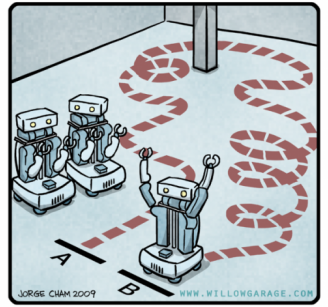
\includegraphics[width=1.0\textwidth, right]{figures/path-planning2}
 	\end{column}
\end{columns}

\end{frame}

\begin{frame}
\frametitle{Decision-Theoretic Planning}
\framesubtitle{Example Domain: Path Planning}
\centering

\begin{columns}[T]
	\begin{column}{.6\textwidth}
		\centering
	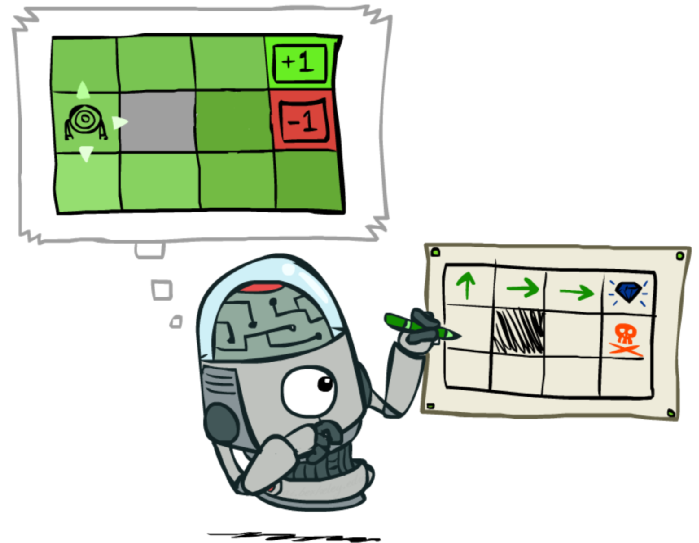
\includegraphics[width=0.7\textwidth]{figures/path-planning3}
	\vfill
	{\tiny Source: \href{http://ai.berkeley.edu/lecture_slides.html}{Berkeley CS188 sheets}}
	\end{column}
	\begin{column}{.5\textwidth}
		\centering
		\vspace{20pt}
		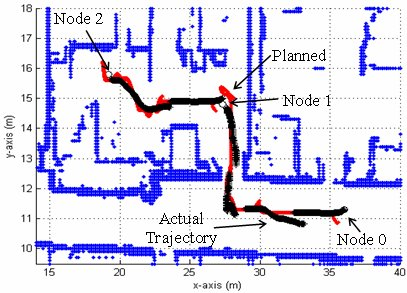
\includegraphics[width=0.75\textwidth]{figures/path-planning4}\\
		\vspace{2.5pt}
		{\tiny Source: \url{http://www.cs.cmu.edu/~gunhee/r\_psr.html}}
	\end{column}
\end{columns}

\end{frame}

\begin{frame}
\frametitle{Decision-Theoretic Planning}
\framesubtitle{Example Domain: Motion Planning}
\begin{center}
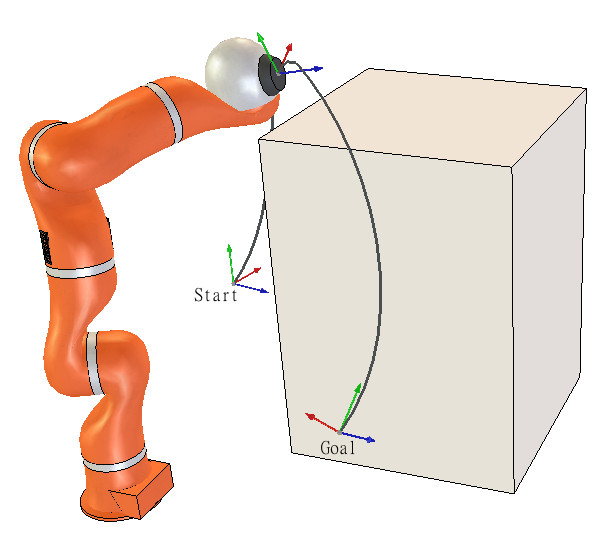
\includegraphics[width=0.38\textwidth]{figures/motion-planning}
\vfill
{\tiny Source: \url{http://www.coppeliarobotics.com/helpFiles/en/motionPlanningModule.htm}}
\end{center}
\end{frame}

\begin{frame}
\frametitle{Decision-Theoretic Planning}
\framesubtitle{Markov Decision Processes (MDPs)}

In DTP systems are modeled by probabilistic models, e.g. MDPs:
\begin{columns}[T]
\begin{column}{0.65\textwidth}
	\begin{definition}
	An MDP is a 5-tuple $\mathcal{M} = (\mathcal{S}, s_0, A, \delta, R)$:
	\begin{itemize}
		\item $\mathcal{S}$ is the state-space, $s_0 \in \mathcal{S}$ the initial state
		\item $A$ is the action-space
		\item $\delta$ is the transition function (N.B.: accounts for uncertainty) % $\delta: S \times S \times A \mapsto [0,1]$
		\item $R$ is the reward function (N.B.: defines the goals)
	\end{itemize}
	\end{definition}
\end{column}

\begin{column}{0.375\textwidth}
	\vspace{32pt}
%	\begin{tikzpicture}[->,>=stealth',auto,node distance=2cm]
%	\tikzstyle{every state}=[fill=white,draw=black,text=black,scale=1, thick]	% thick
%	\node[state] (s1) {$q_t$};
%	\node[state] (s2) [right of=s1] {$q_{t+1}$};
%	\path
%	(s1)
%	edge node {} (s2)
%	(s2);
%	;
%	\end{tikzpicture}
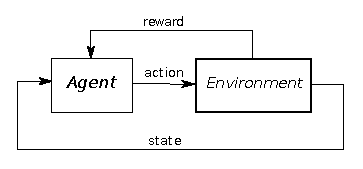
\includegraphics{figures/mdp}
\end{column}
\end{columns}
\end{frame}

\begin{frame}
\frametitle{Decision-Theoretic Planning}
\framesubtitle{Learning Optimal Plans}

\begin{center}
	\vspace{-12pt}
	\includegraphics<1| handout:0>[width=0.95\textwidth]{figures/planning-routine/mdp-planning-diagram-v2-1x.pdf}
	\includegraphics<2|handout:0>[width=0.95\textwidth]{figures/planning-routine/mdp-planning-diagram-v2-2.pdf}
	\includegraphics<3|handout:0>[width=0.95\textwidth]{figures/planning-routine/mdp-planning-diagram-v2-3.pdf}
	\includegraphics<4|handout:0>[width=0.95\textwidth]{figures/planning-routine/mdp-planning-diagram-v2-4.pdf}
	\includegraphics<5>[width=0.95\textwidth]{figures/planning-routine/mdp-planning-diagram-v2-5.pdf}
\end{center}

\end{frame}

\begin{frame}
\frametitle{Decision-Theoretic Planning}

%\begin{center}
	\textcolor{tudBlack}{\textbf{Problem:}} How to find a suitable MDP model?
	\pause
	\vfill
	\textcolor{tudBlack}{\textbf{Classical approach:}} Model development by a \textit{human designer}, however:
	\begin{itemize}
		\item Requires significant effort (e.g., trial-and-error)
		\item Typically demands knowledge/experience, accompanied by high costs
	\end{itemize}
	\pause
%	\vfill
%	\textcolor{black}{\textbf{Alternative:}} Use reinforcement learning
	\vfill
	\textcolor{tudBlack}{\textbf{Idea:}} Automate the model building process by learning algorithms 
	\begin{itemize}
		\item Learn from (exploration) data about the environment
		\item Optimization for the best MDP model
	\end{itemize}
%\end{center}

\end{frame}

\section{Model Optimization}

\begin{frame}
\frametitle{Mobile Robot Navigation}
\textcolor{tudblue}{\textbf{Goal:}} Move robot to area while minimizing traveled distance
\vfill

\begin{columns}[T]
\begin{column}{0.6\textwidth}
MDP Model $\mathcal{M}$ should define:
\begin{itemize}
	\item Attainable states, corresponding to locations
	\item Possible actions, robot translations
\end{itemize}
\end{column}

\begin{column}{0.4\textwidth}
	
\end{column}

\end{columns}

\end{frame}

\begin{frame}
\frametitle{Model-Learning for Mobile Robot Navigation}

\begin{columns}[T]
\begin{column}{0.6\textwidth}
\begin{itemize}
	\item \textbf{TODO}
	\item[] 
	\item Simulation in Morse with a Scitos A5 robot
\end{itemize}
\end{column}
\begin{column}{0.5\textwidth}
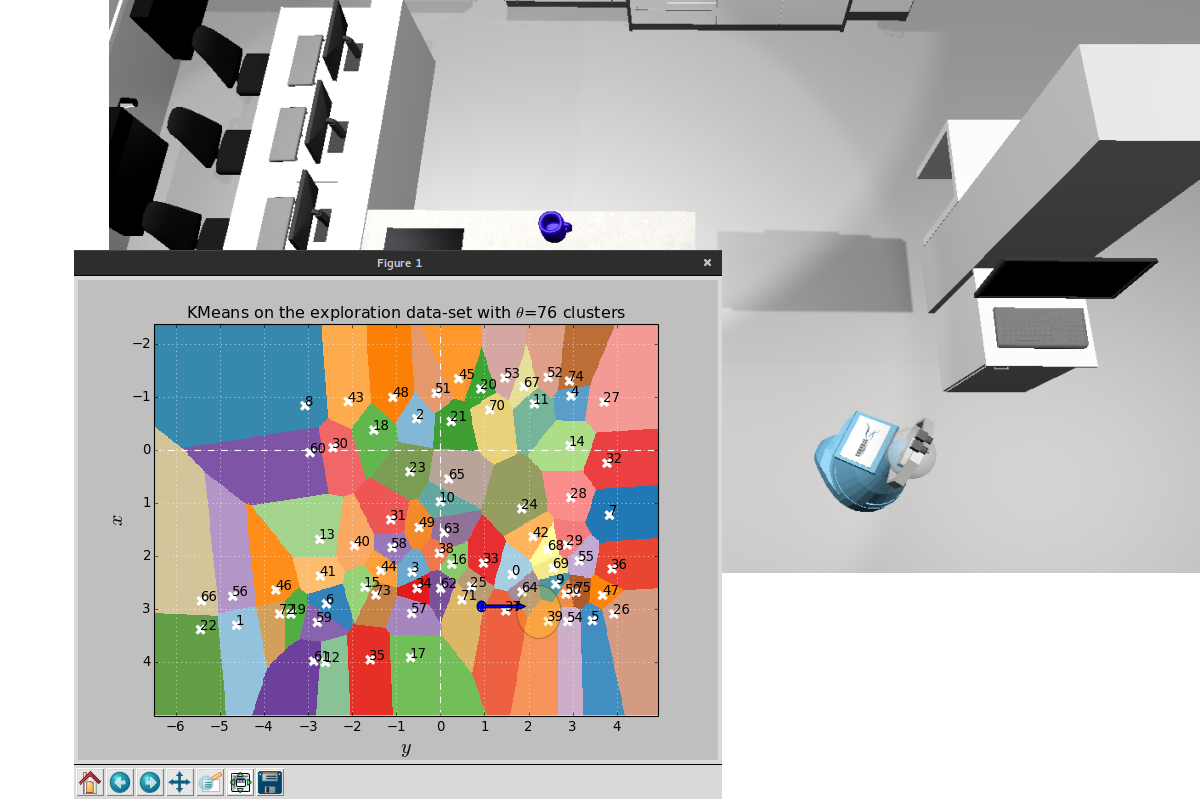
\includegraphics[width=\textwidth, left]{figures/simulation_learn_2}
\end{column}
\end{columns}	
	
\end{frame}

\begin{frame}
\frametitle{Model-Optimization Routine}
\begin{center}
\includegraphics<1| handout:0>[width=1\textwidth]{figures/optimization-routine/learning-cycle-1.pdf}
\includegraphics<2| handout:0>[width=1\textwidth]{figures/optimization-routine/learning-cycle-2.pdf}
\includegraphics<3| handout:0>[width=1\textwidth]{figures/optimization-routine/learning-cycle-3.pdf}
\includegraphics<4| handout:0>[width=1\textwidth]{figures/optimization-routine/learning-cycle-4.pdf}
\includegraphics<5>[width=1\textwidth]{figures/optimization-routine/learning-cycle-5.pdf}
\end{center}
\end{frame}

\begin{frame}
\frametitle{Model-Optimization Routine}
\begin{center}
	\includegraphics<1| handout:0>[width=1\textwidth]{figures/optimization-routine/learning-cycle-simplified-1.pdf}
	\includegraphics<2| handout:0>[width=1\textwidth]{figures/optimization-routine/learning-cycle-simplified-2.pdf}
	\includegraphics<3>[width=1\textwidth]{figures/optimization-routine/learning-cycle-simplified-3.pdf}
\end{center}
\end{frame}

\section{Bayesian Optimization}

\begin{frame}
\frametitle{Bayesian Optimization}

\begin{itemize}
	\item \textbf{TODO}
\end{itemize}
\end{frame}

\begin{frame}
\frametitle{Bayesian Optimization}
\framesubtitle{Example}

\centering
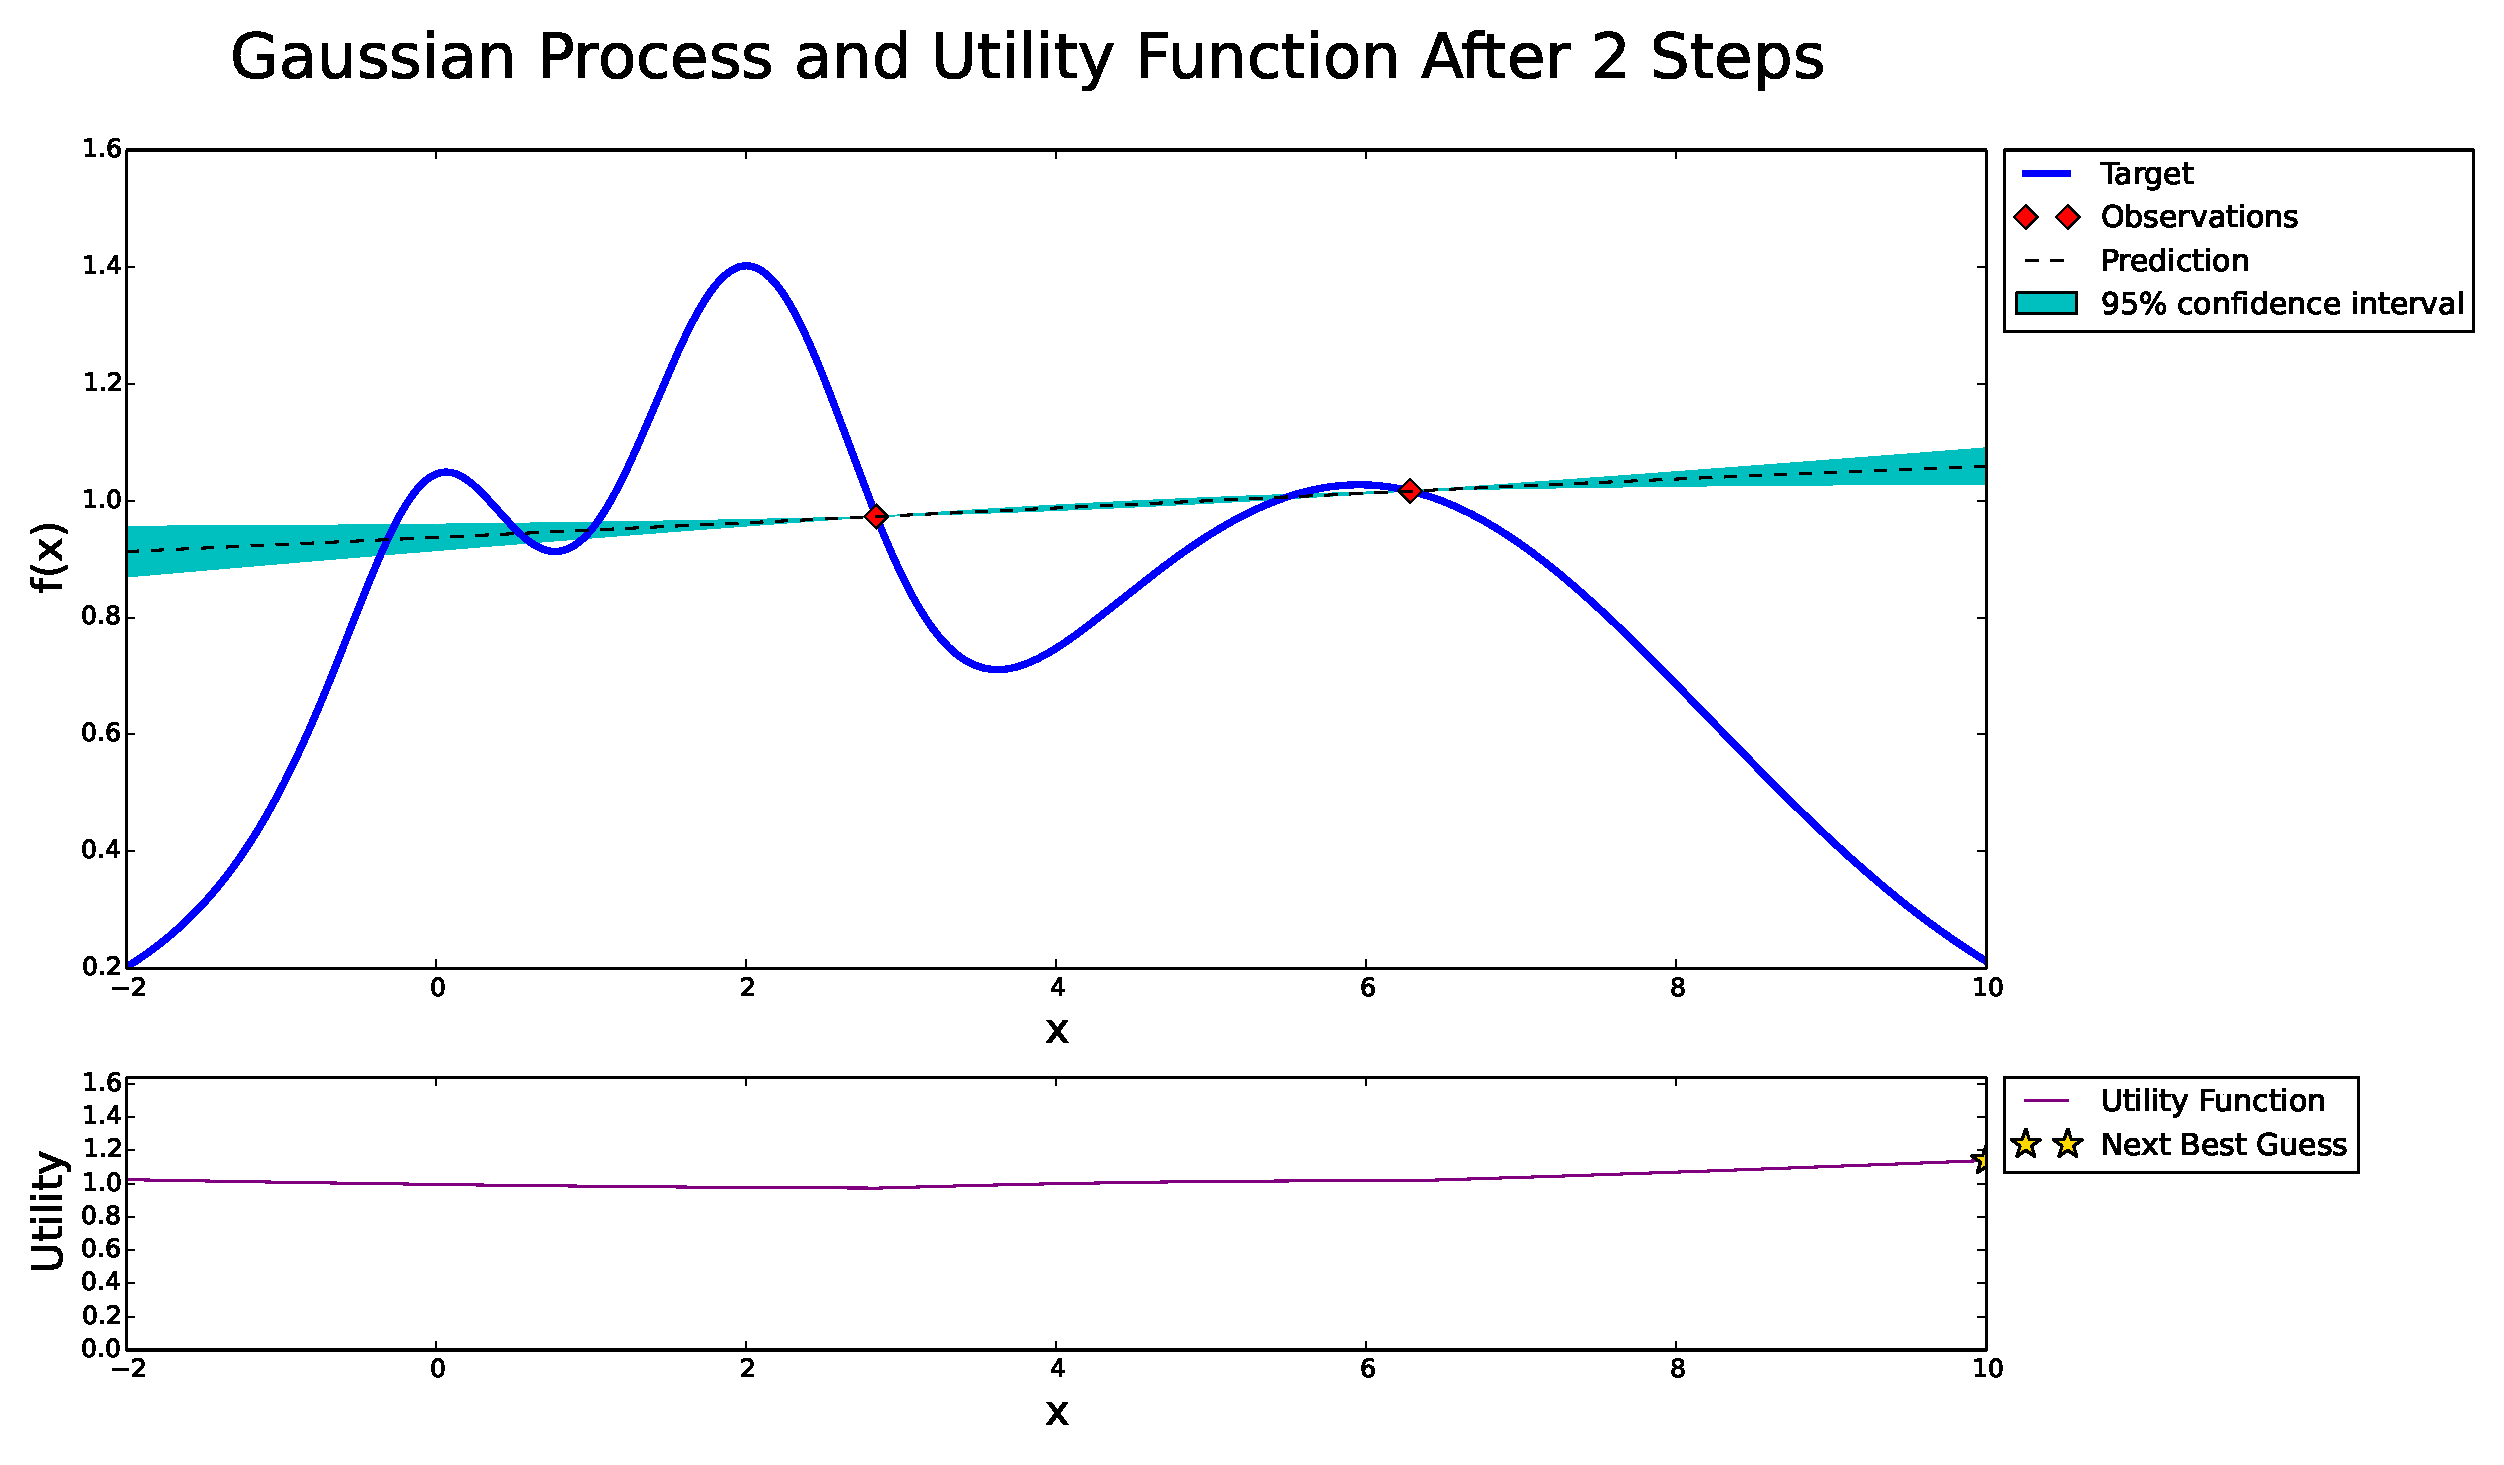
\includegraphics[width=0.8\textwidth]{figures/bayesian-optimization/fig0}

\end{frame}

\begin{frame}
	\frametitle{Bayesian Optimization}
	\framesubtitle{Example}
	
	\centering
	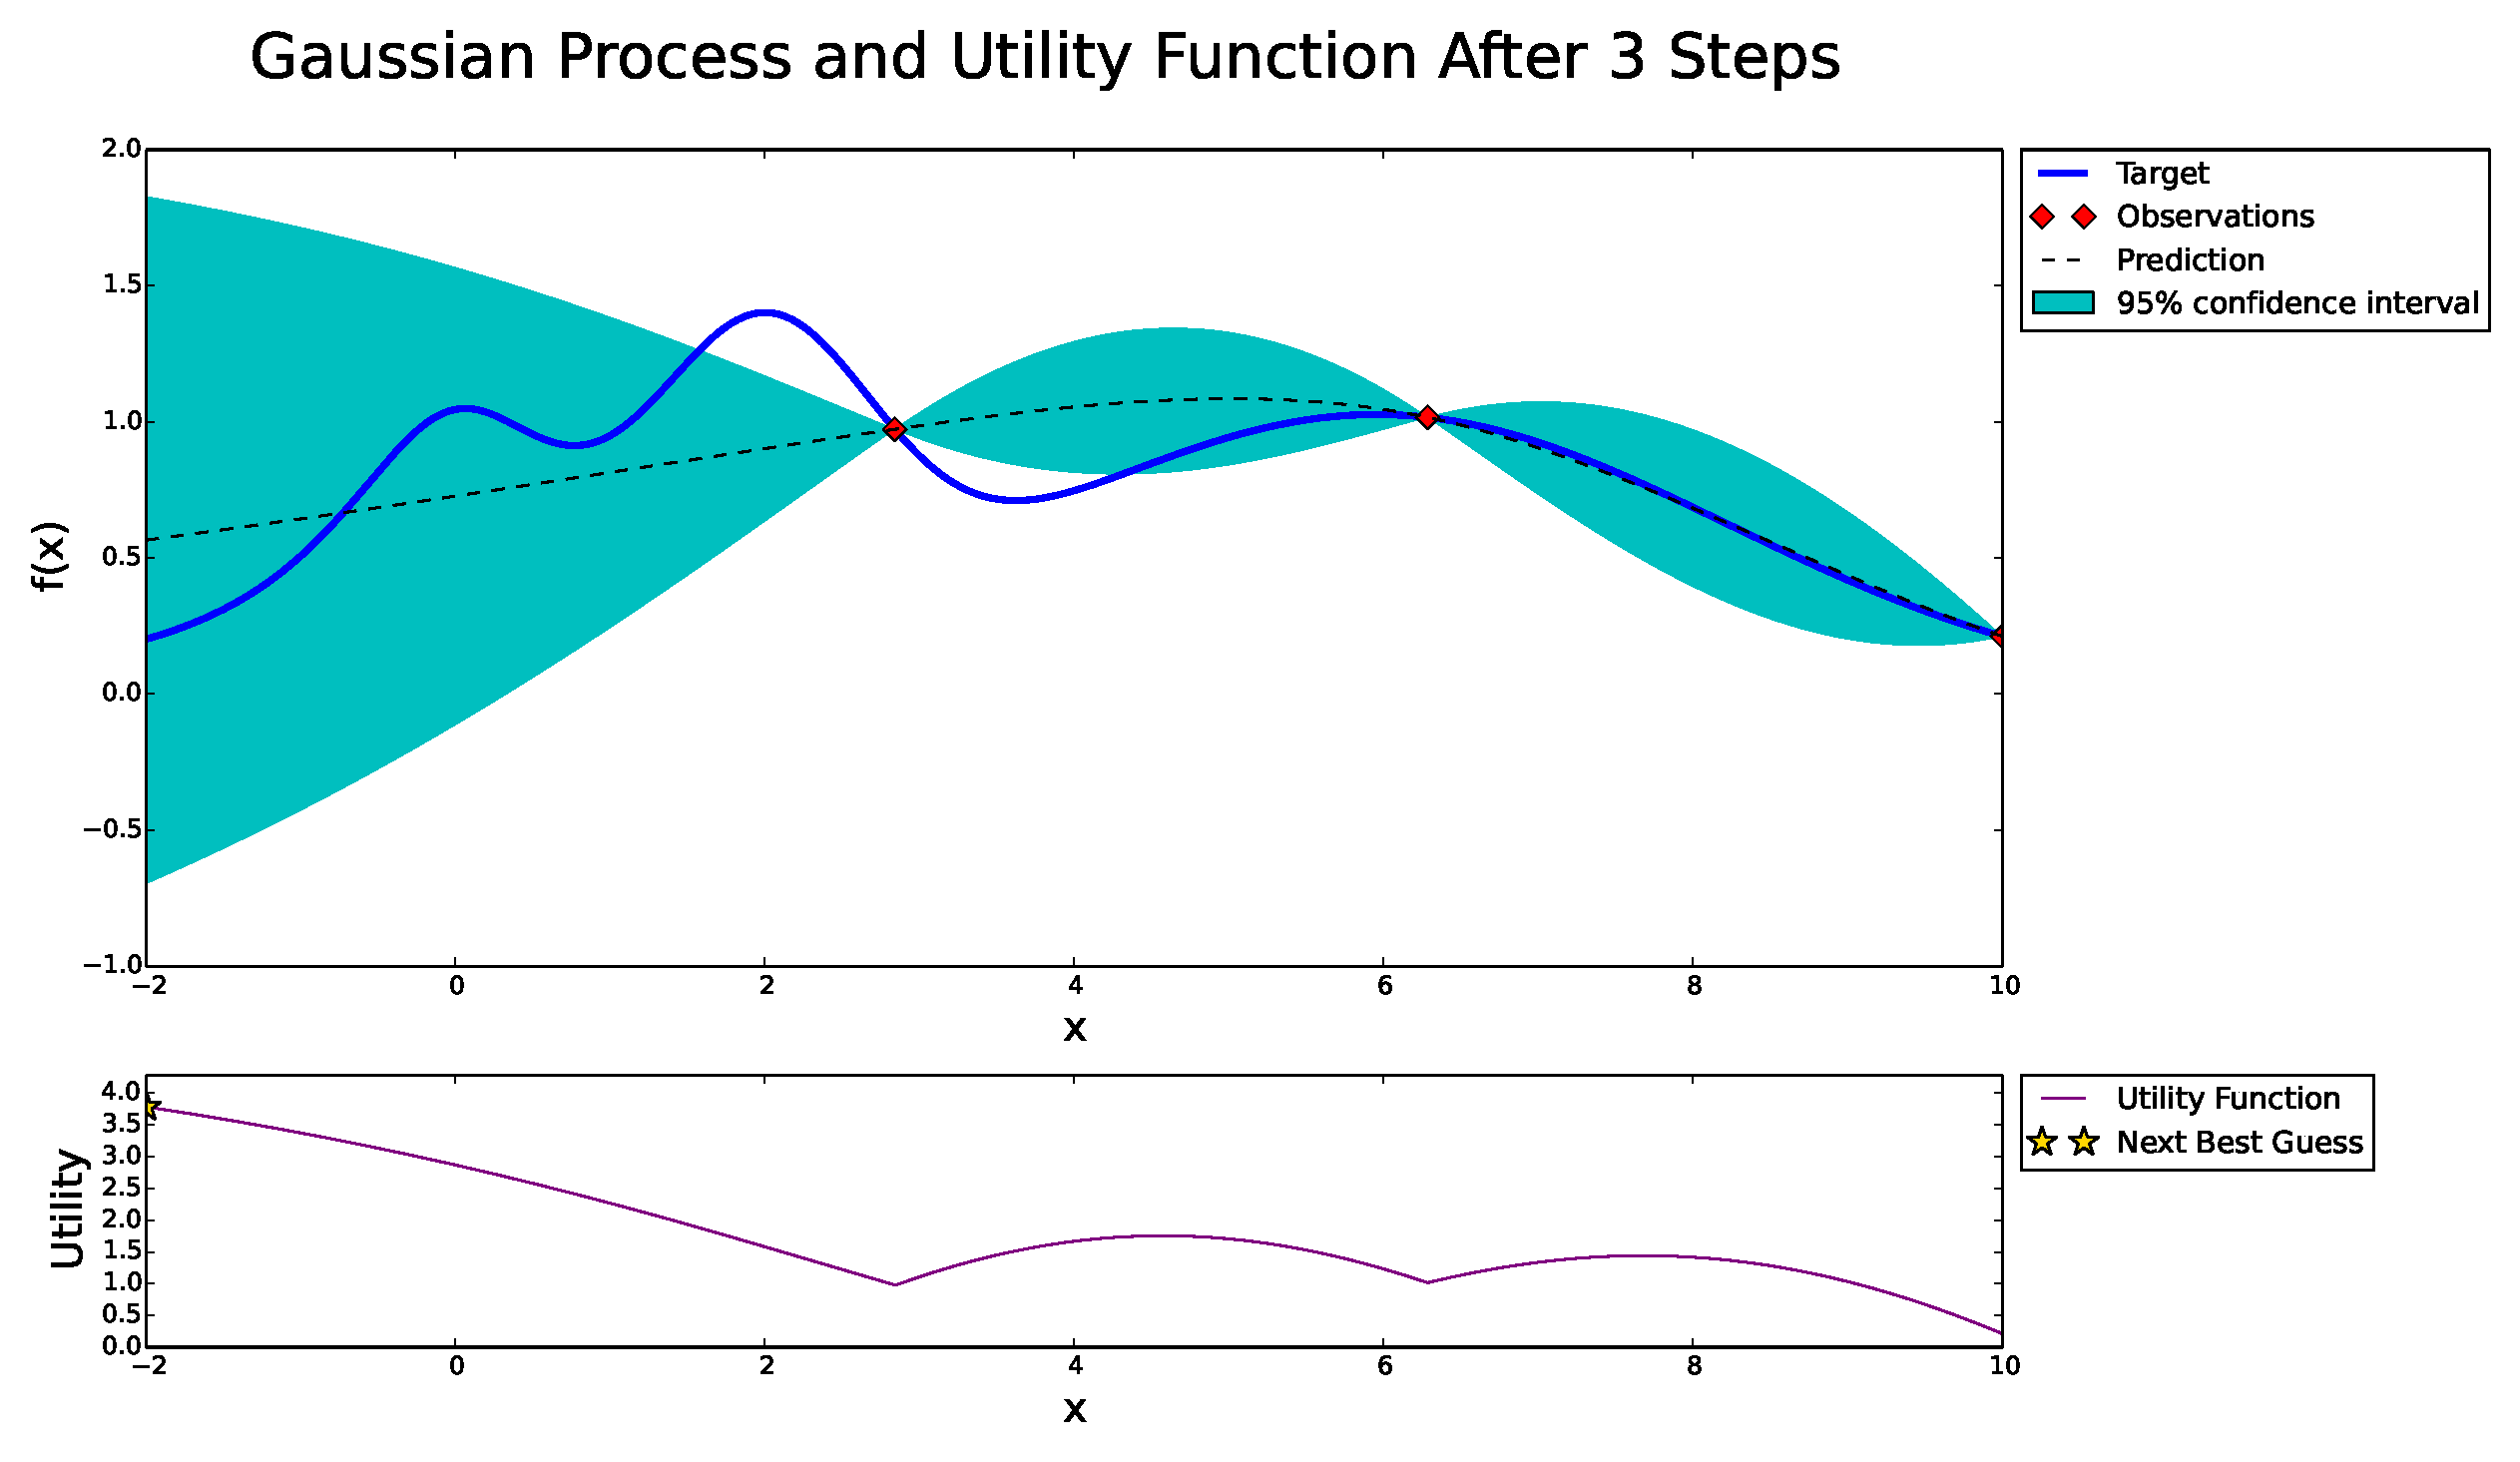
\includegraphics[width=0.8\textwidth]{figures/bayesian-optimization/fig1}
	
\end{frame}

\begin{frame}
	\frametitle{Bayesian Optimization}
	\framesubtitle{Example}
	
	\centering
	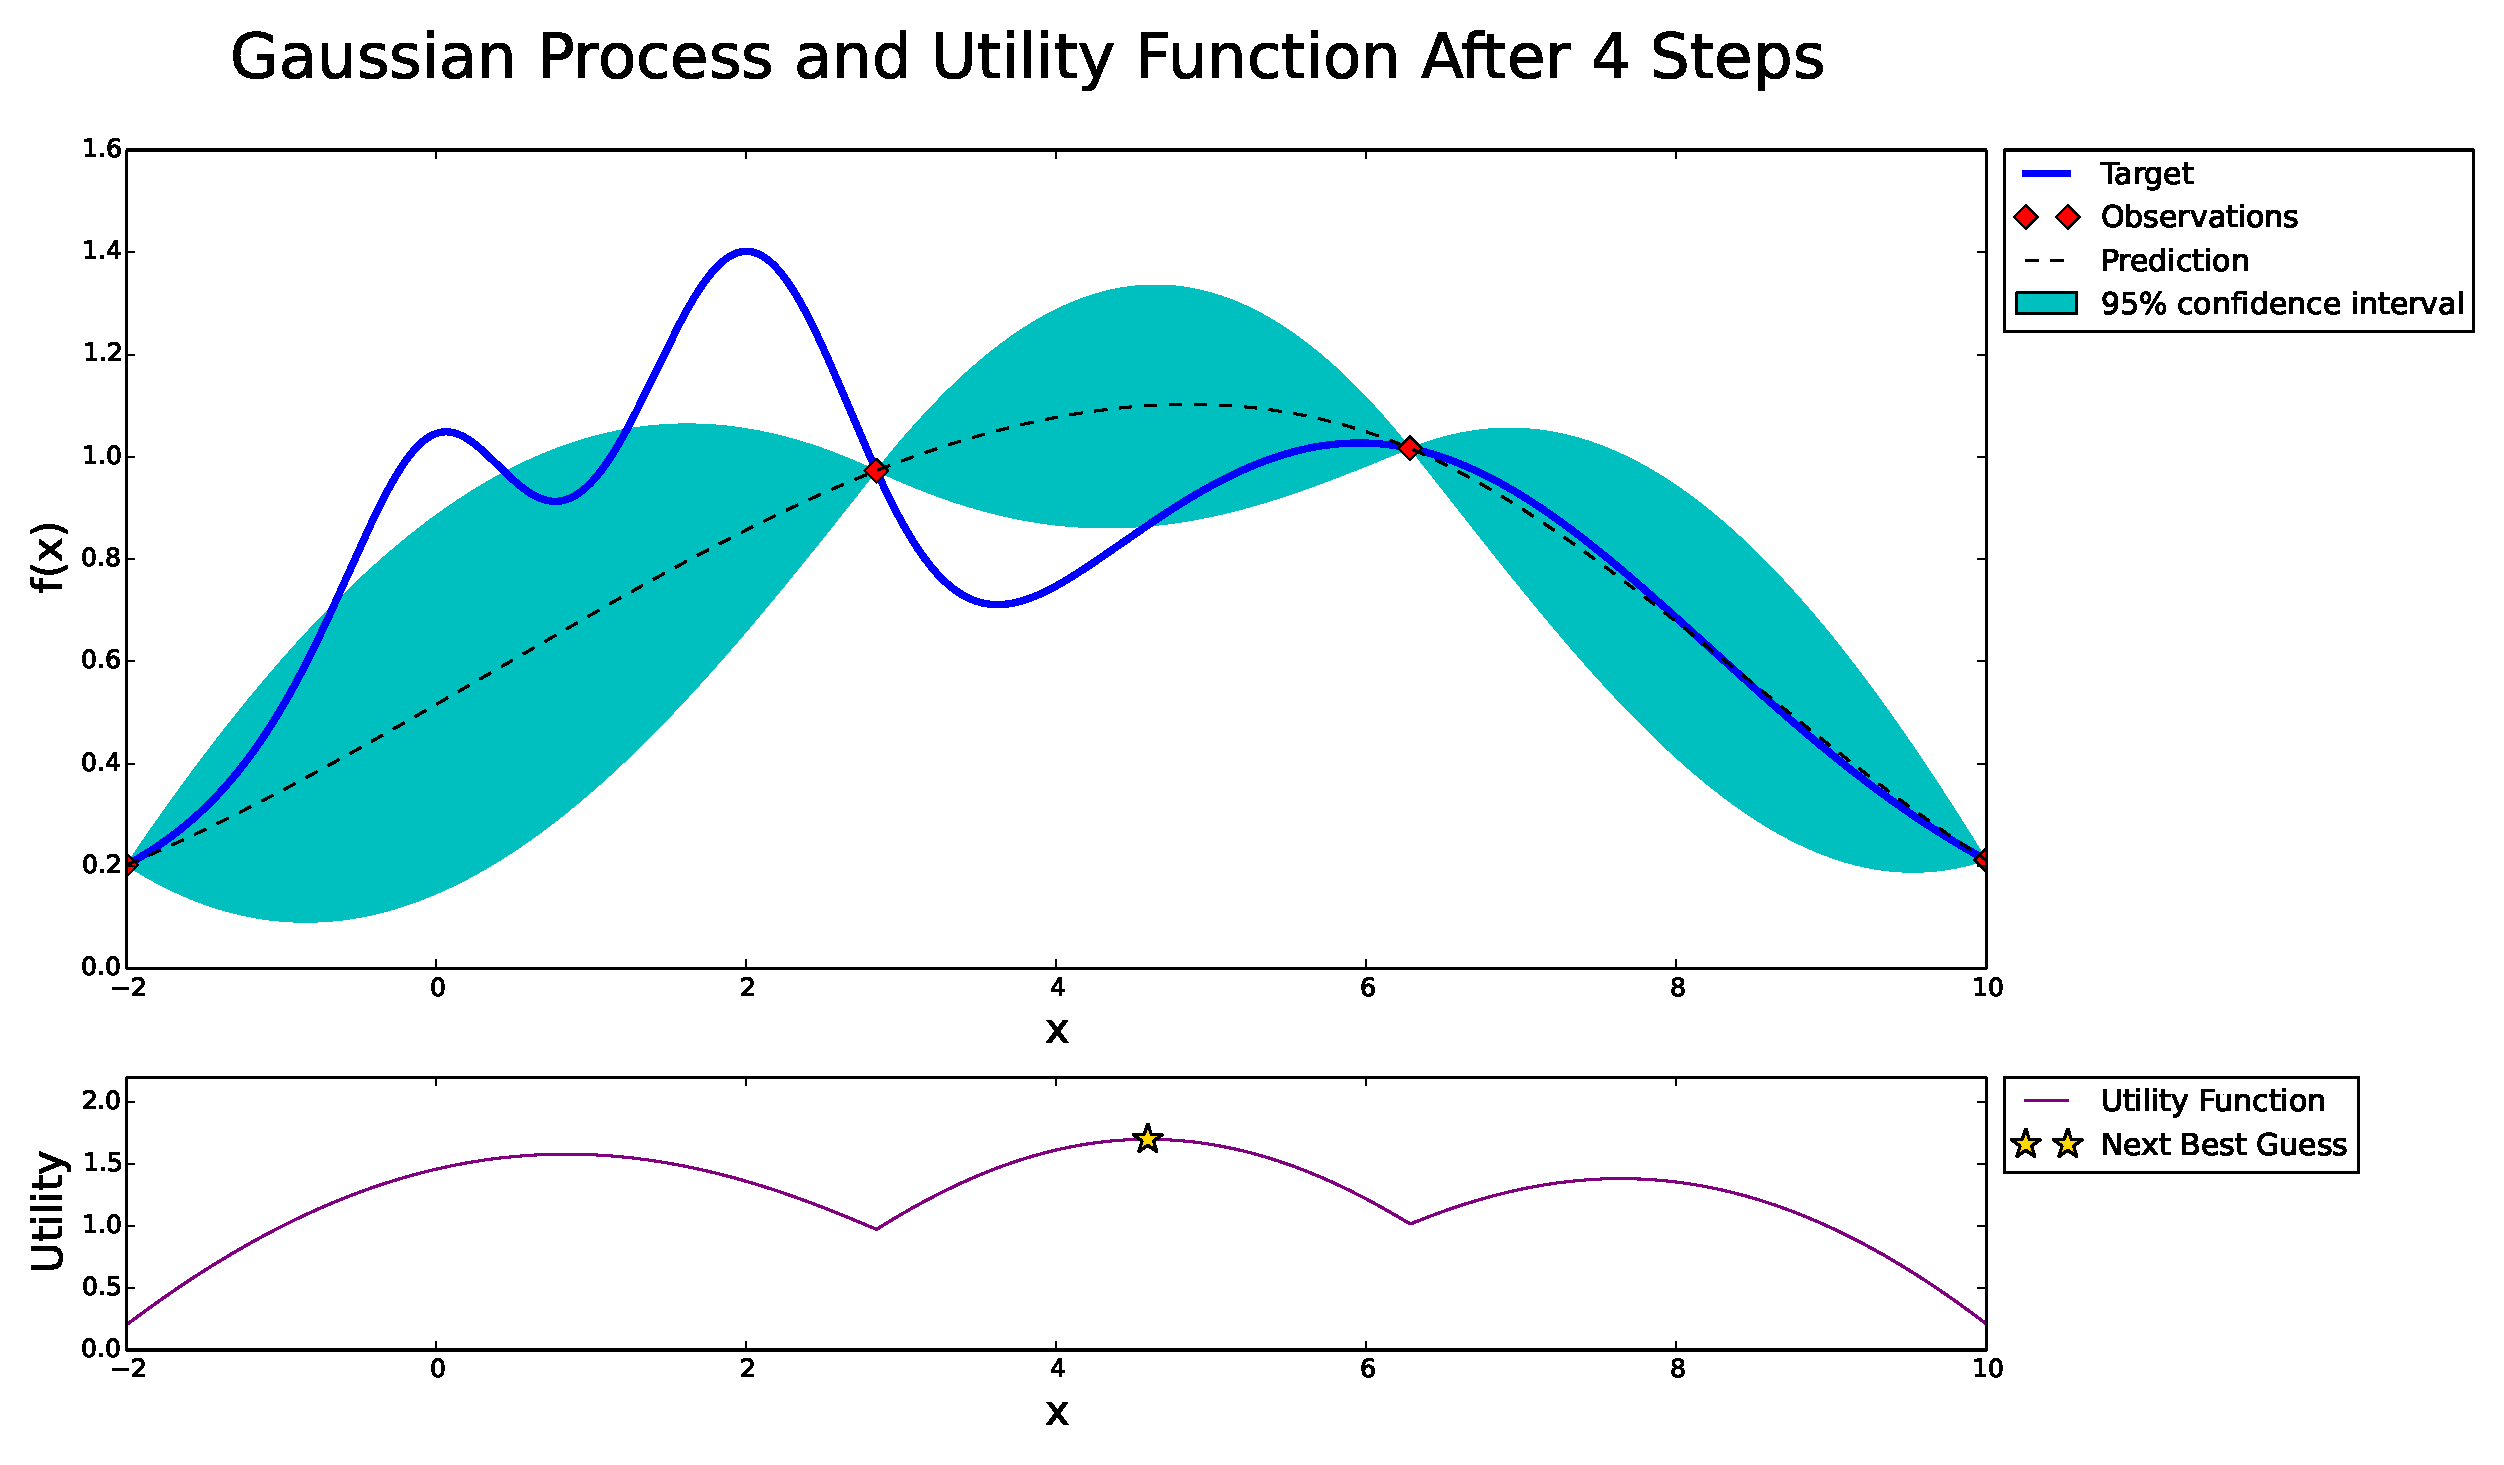
\includegraphics[width=0.8\textwidth]{figures/bayesian-optimization/fig2}
	
\end{frame}

\begin{frame}
	\frametitle{Bayesian Optimization}
	\framesubtitle{Example}
	
	\centering
	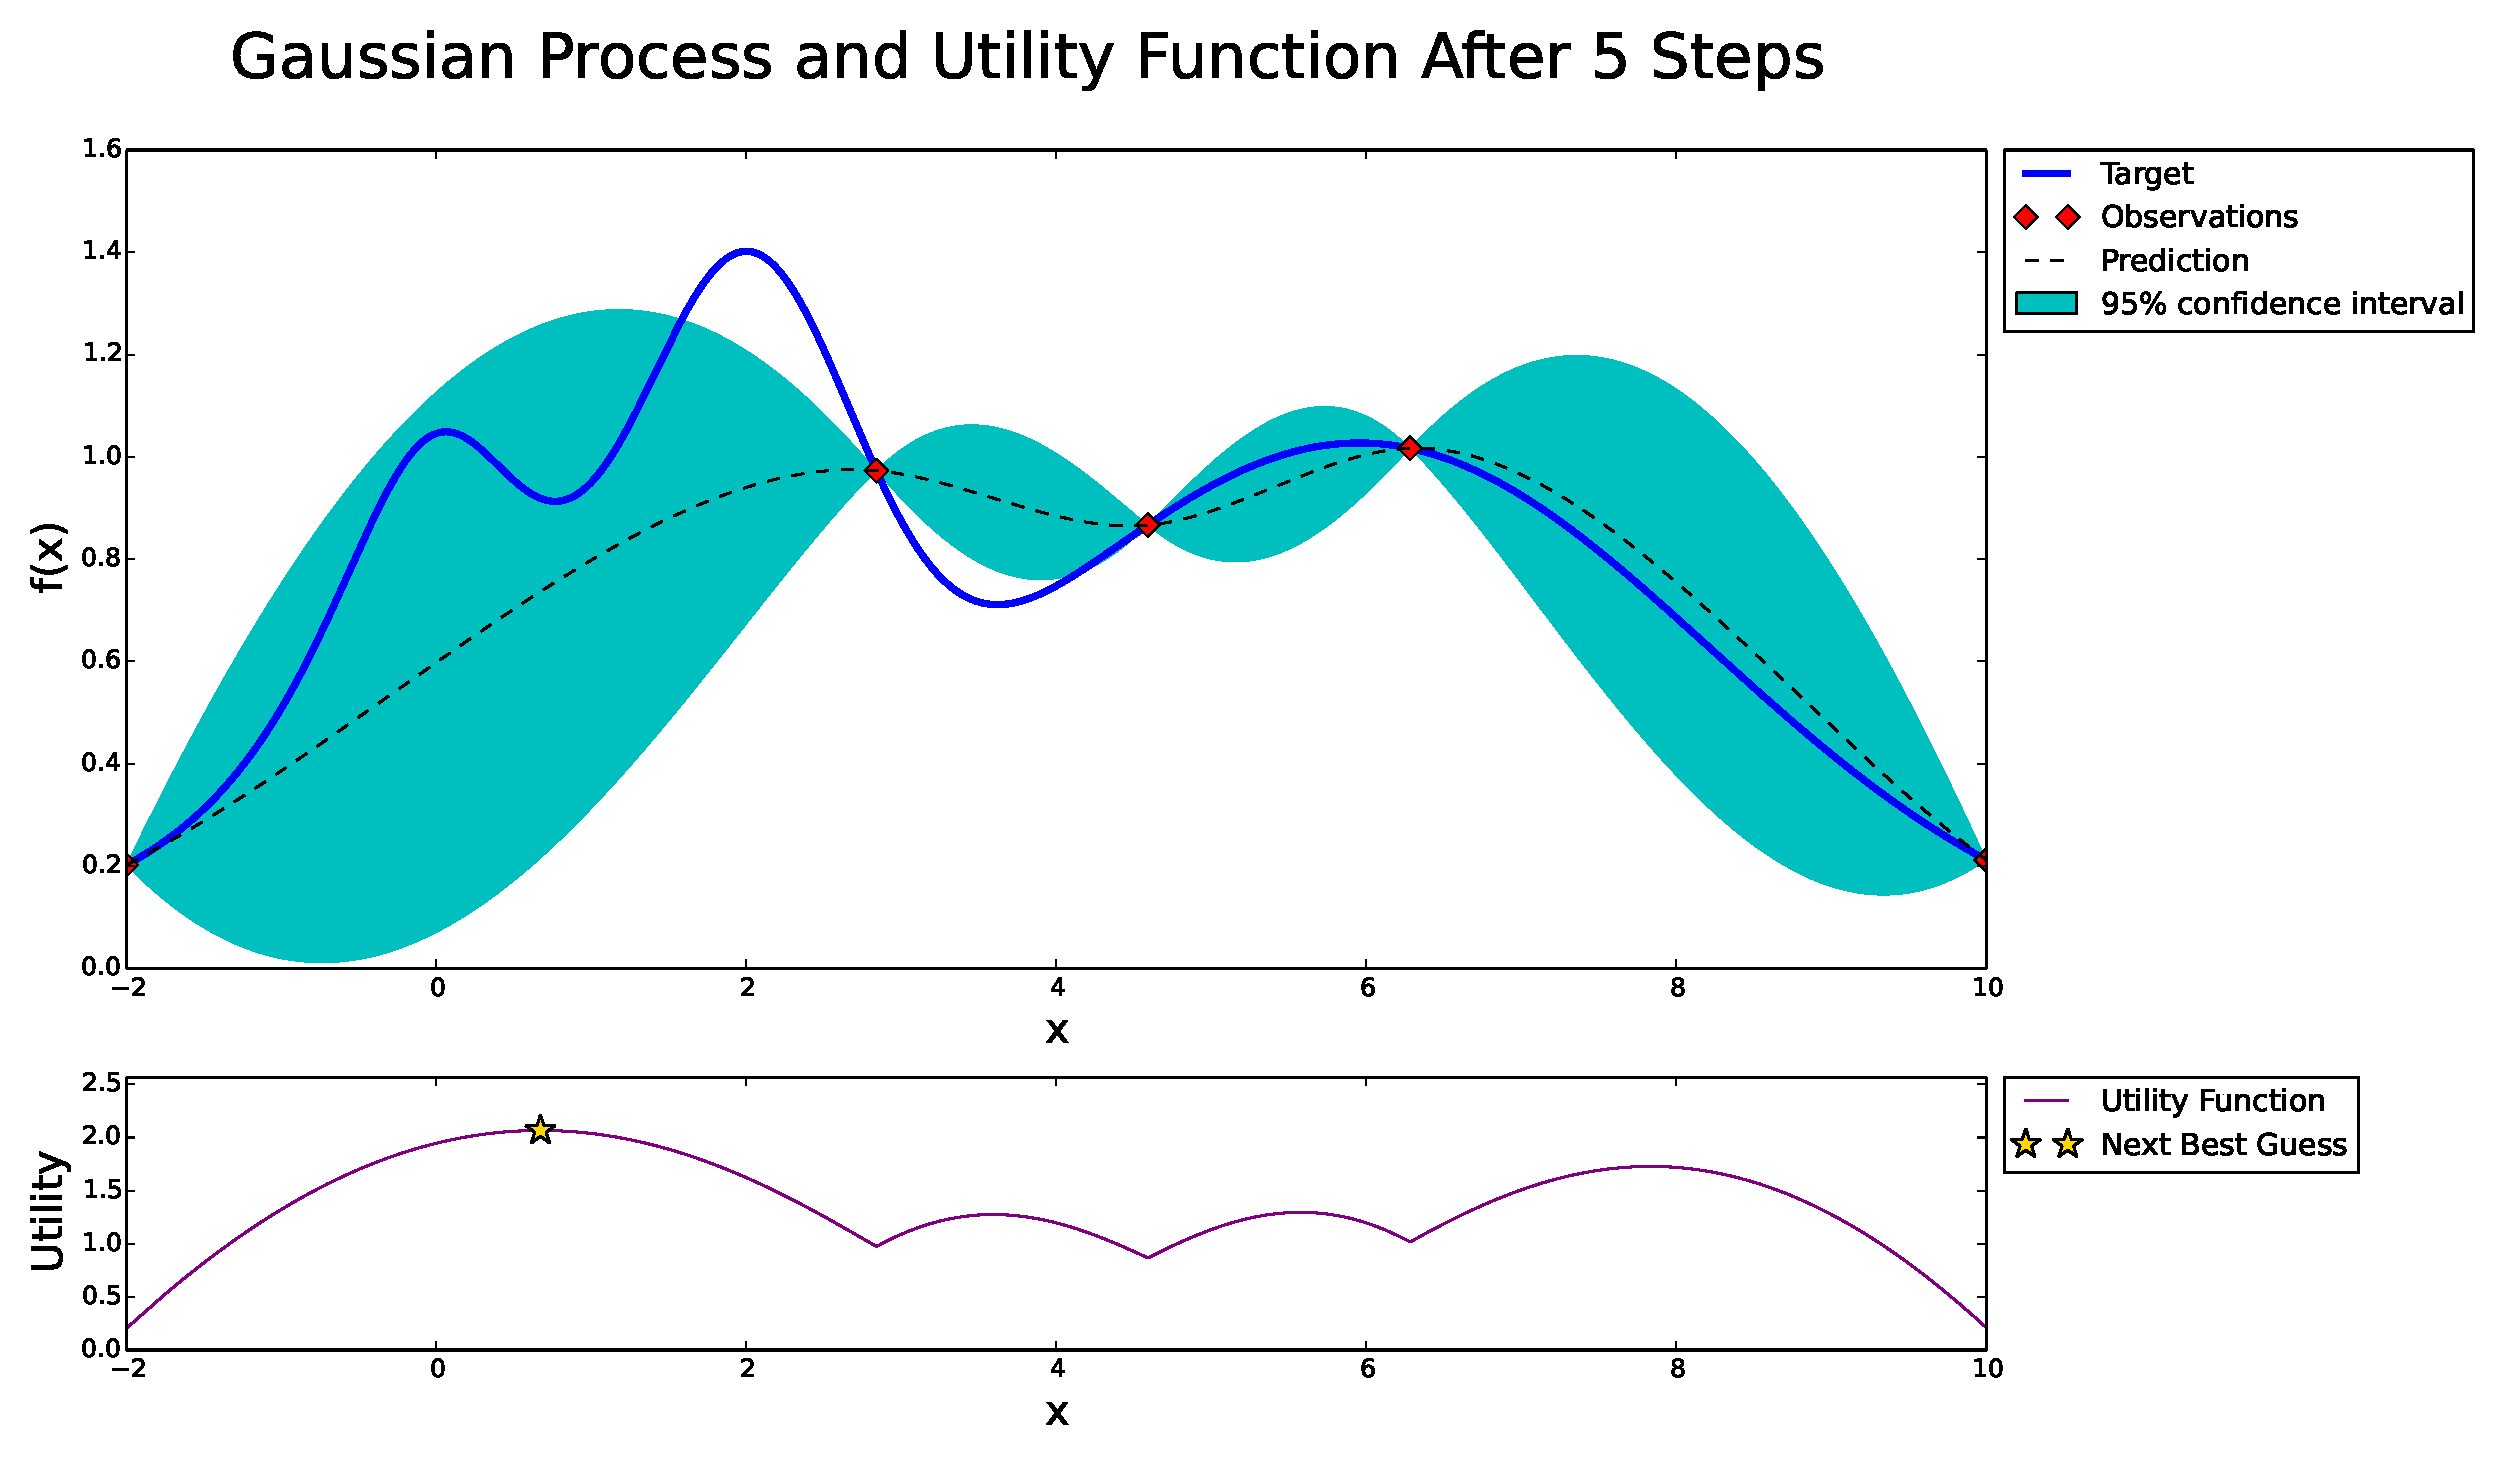
\includegraphics[width=0.8\textwidth]{figures/bayesian-optimization/fig3}
	
\end{frame}

\begin{frame}
	\frametitle{Bayesian Optimization}
	\framesubtitle{Example}
	
	\centering
	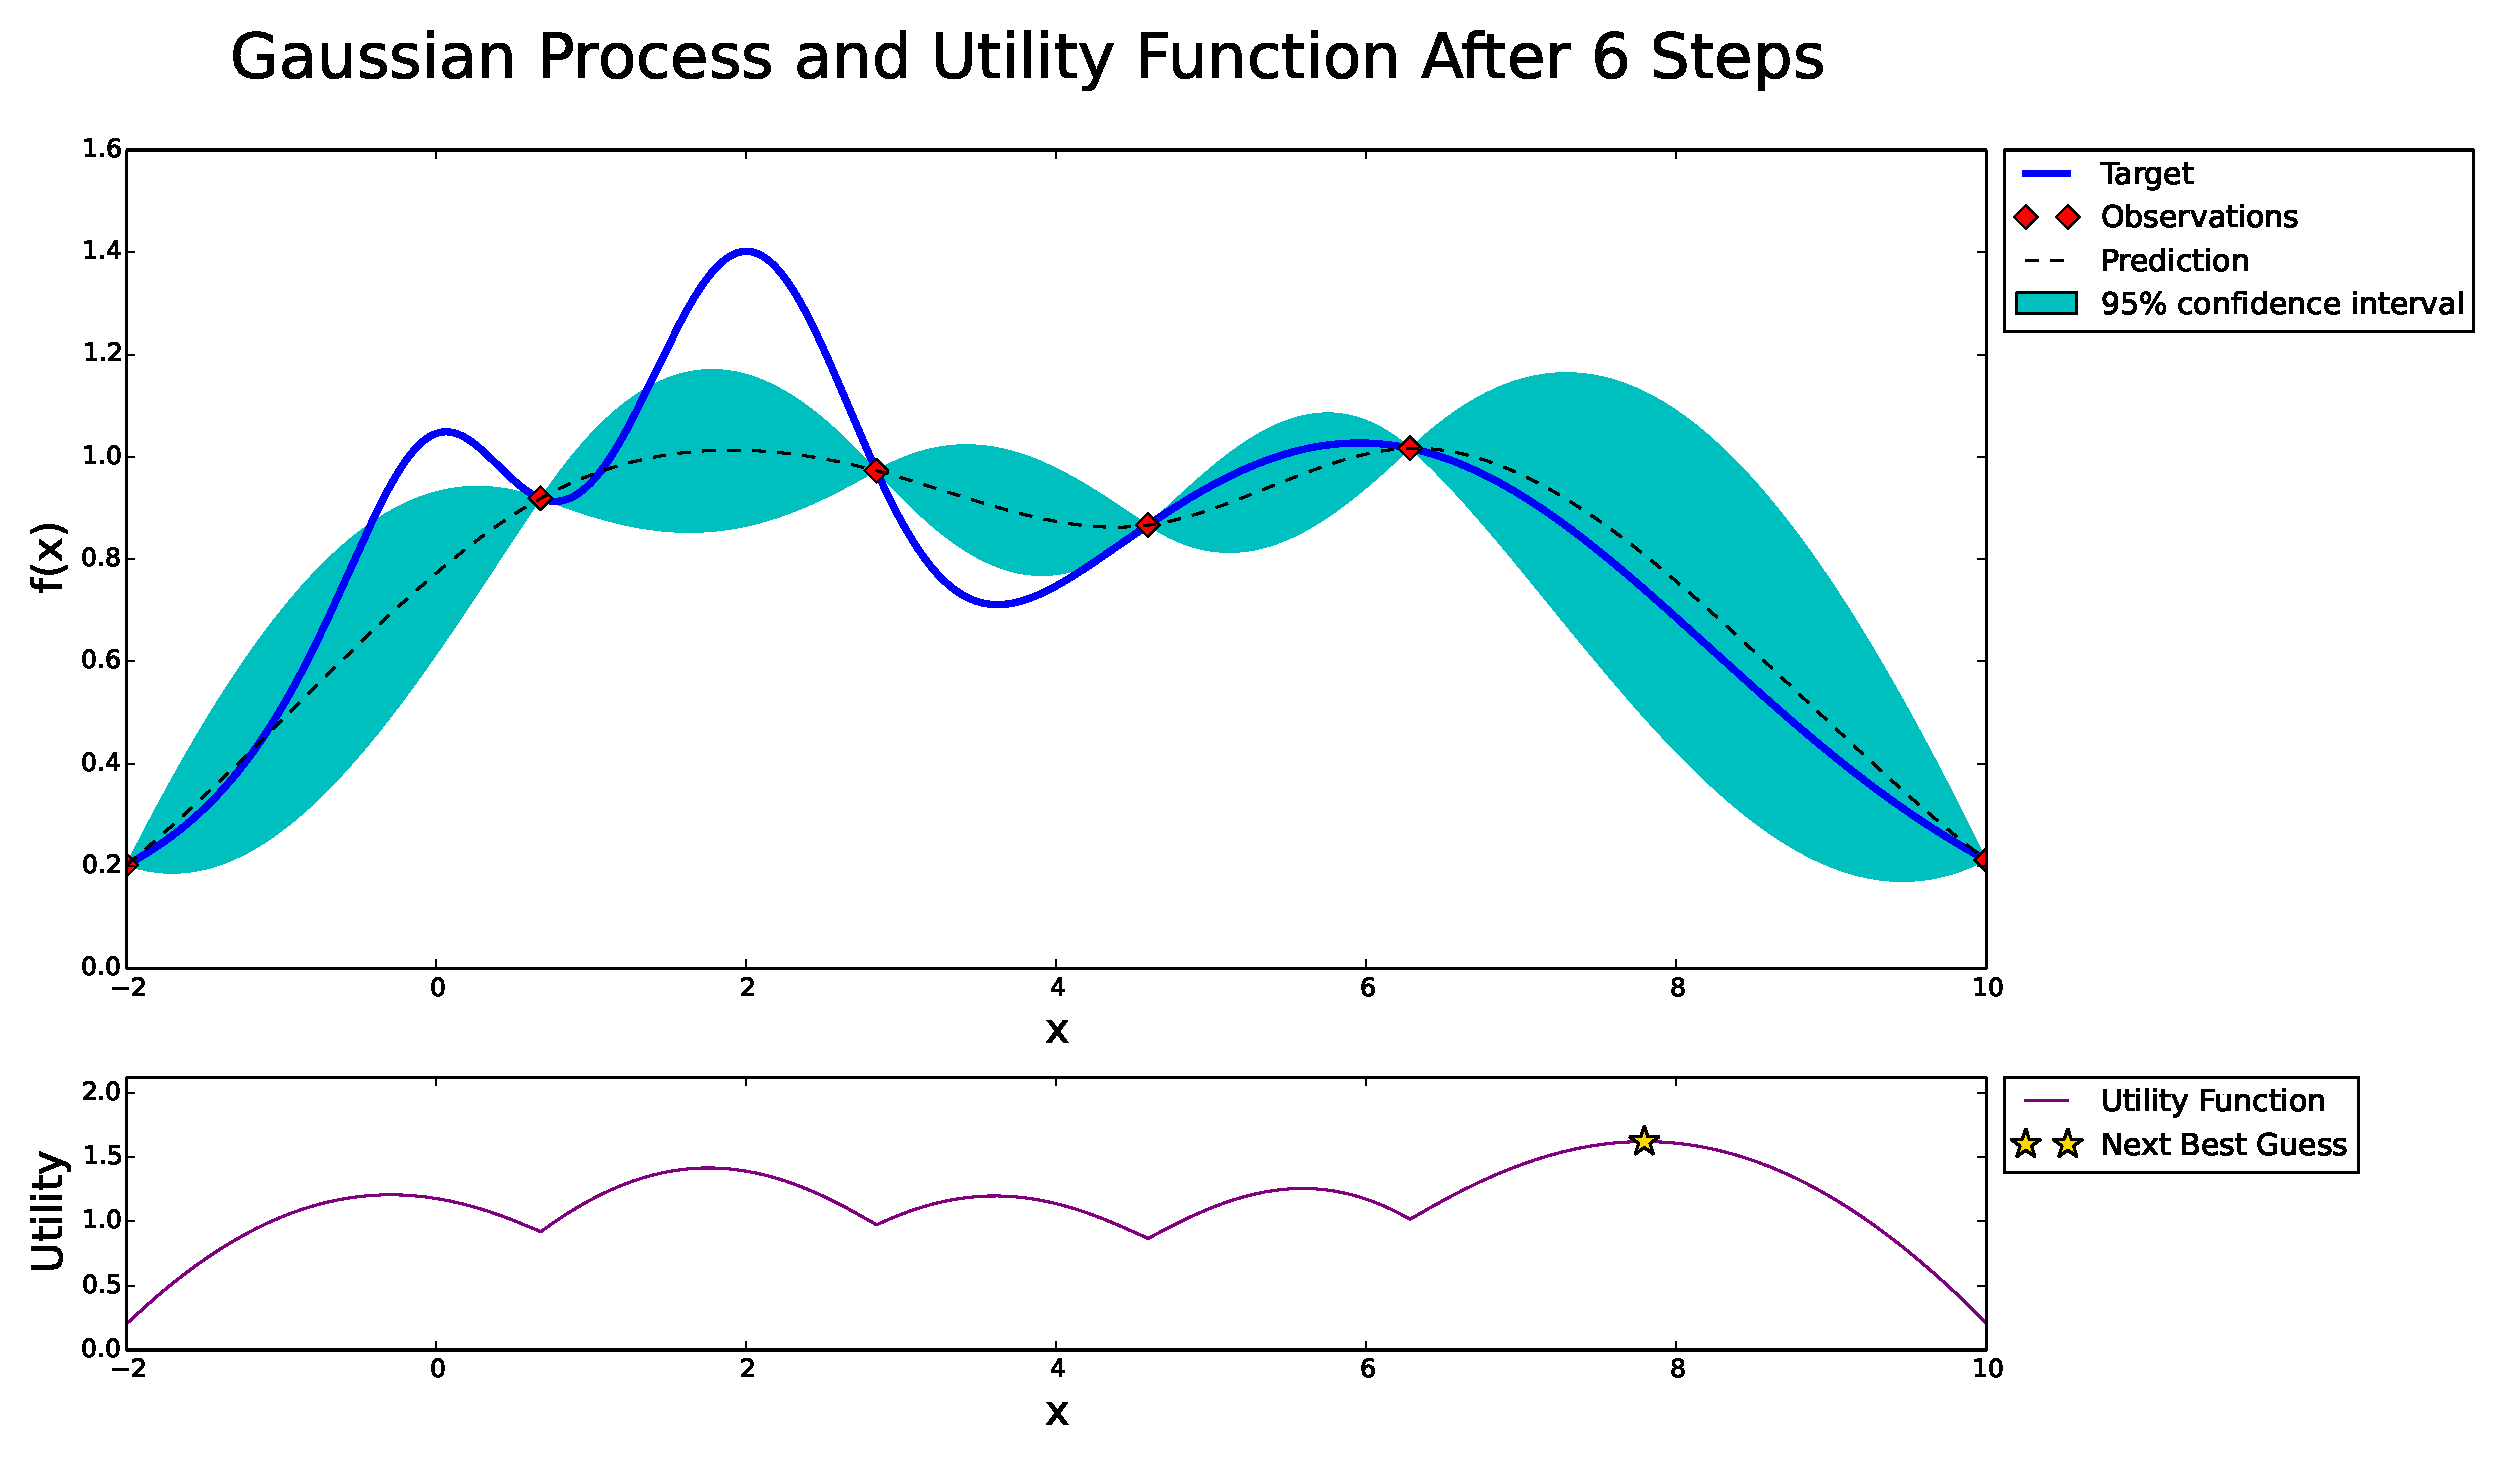
\includegraphics[width=0.8\textwidth]{figures/bayesian-optimization/fig4}
	
\end{frame}

\begin{frame}
	\frametitle{Bayesian Optimization}
	\framesubtitle{Example}
	
	\centering
	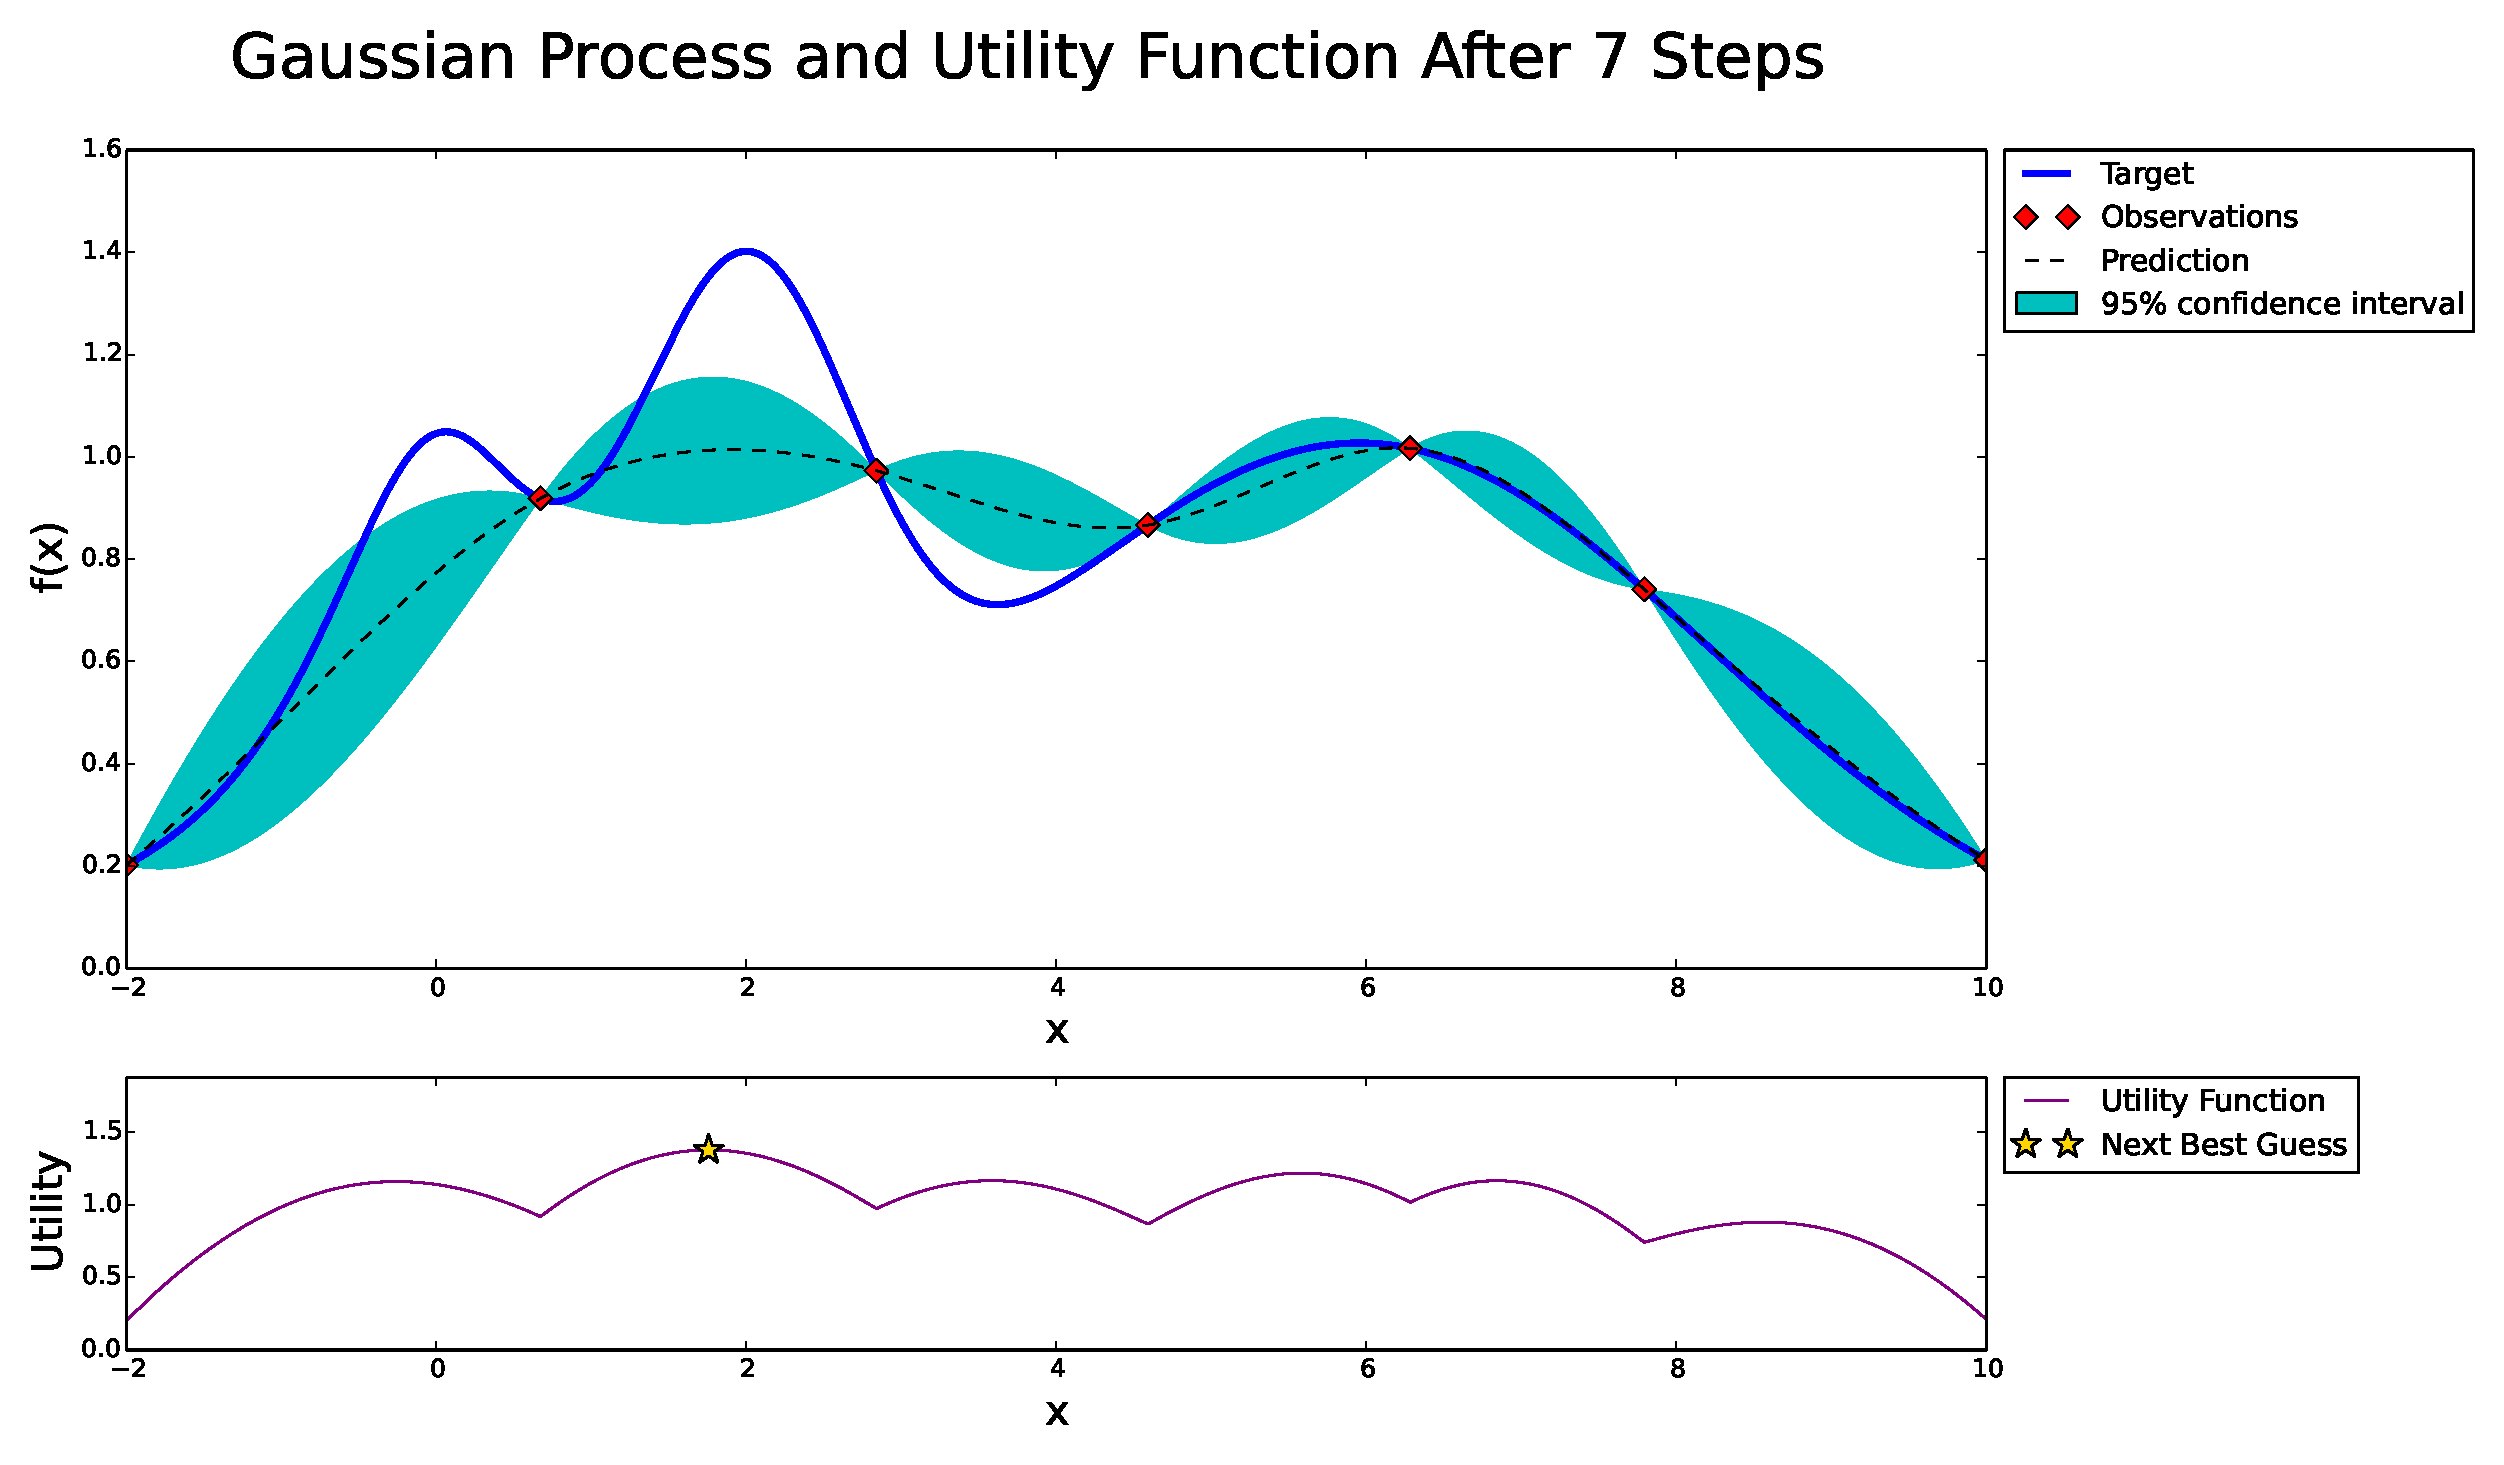
\includegraphics[width=0.8\textwidth]{figures/bayesian-optimization/fig5}
	
\end{frame}

\begin{frame}
	\frametitle{Bayesian Optimization}
	\framesubtitle{Example}
	
	\centering
	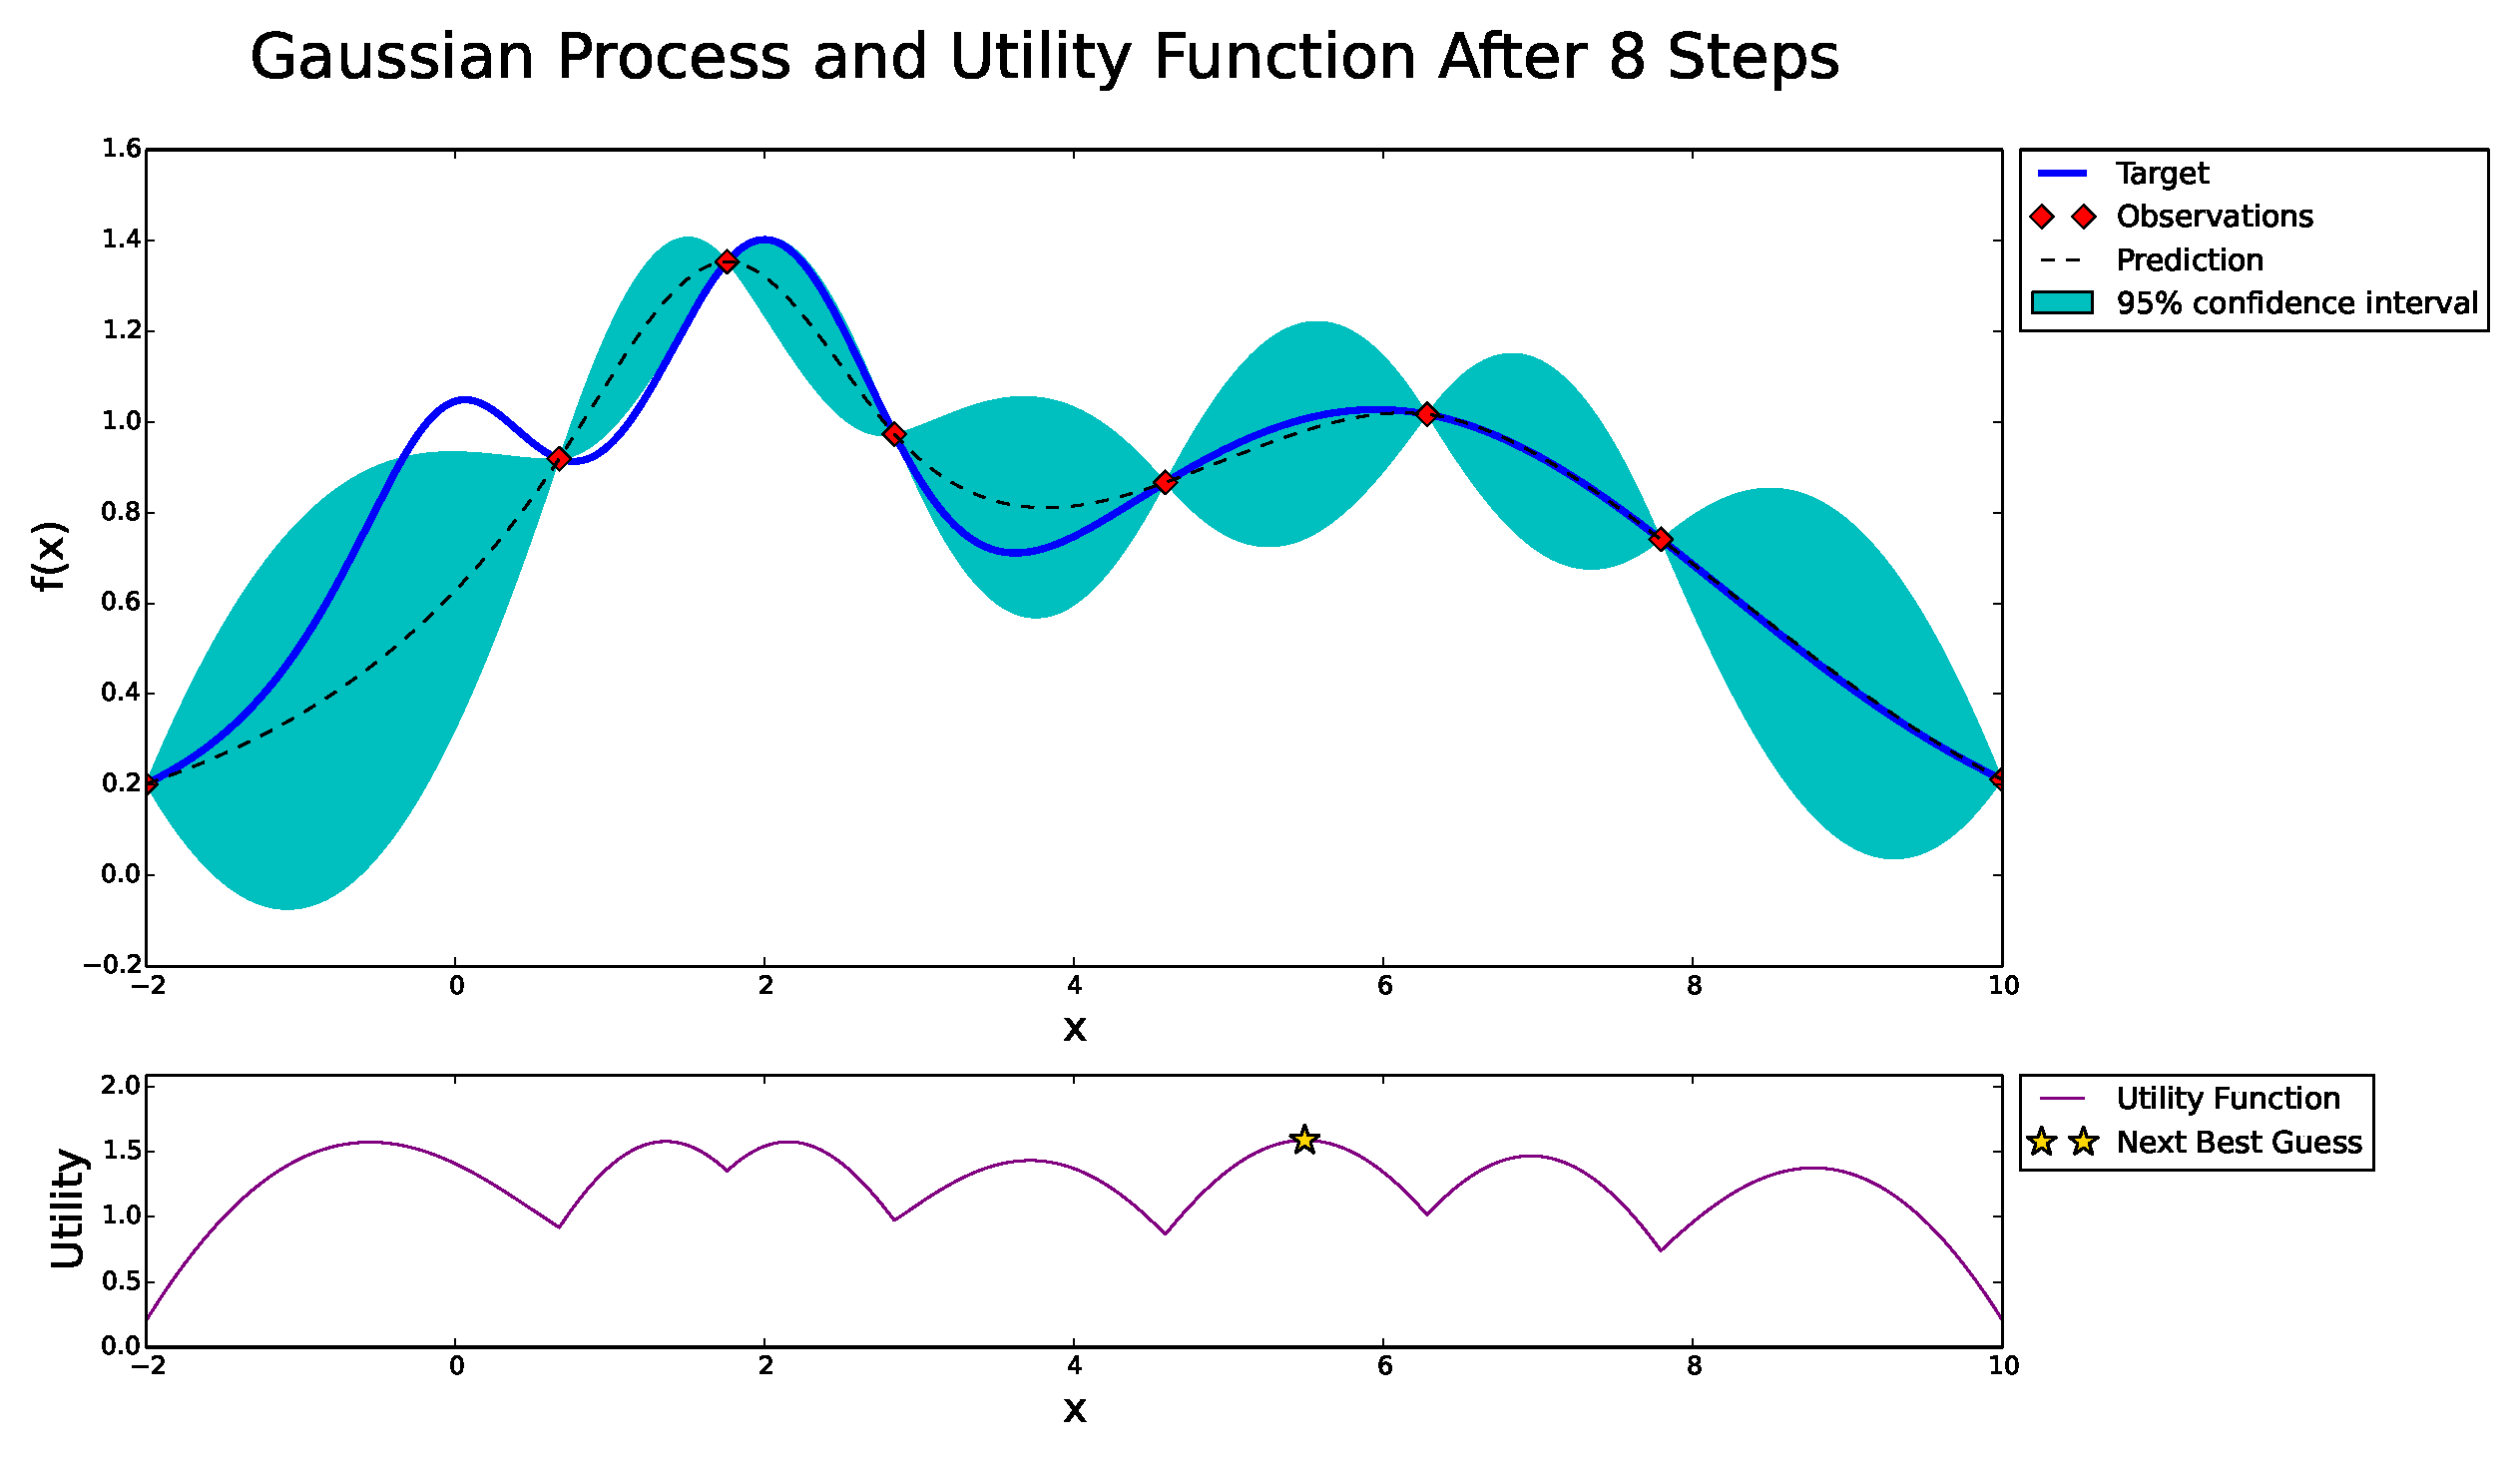
\includegraphics[width=0.8\textwidth]{figures/bayesian-optimization/fig6}
	
\end{frame}

\begin{frame}
	\frametitle{Bayesian Optimization}
	\framesubtitle{Example}
	
	\centering
	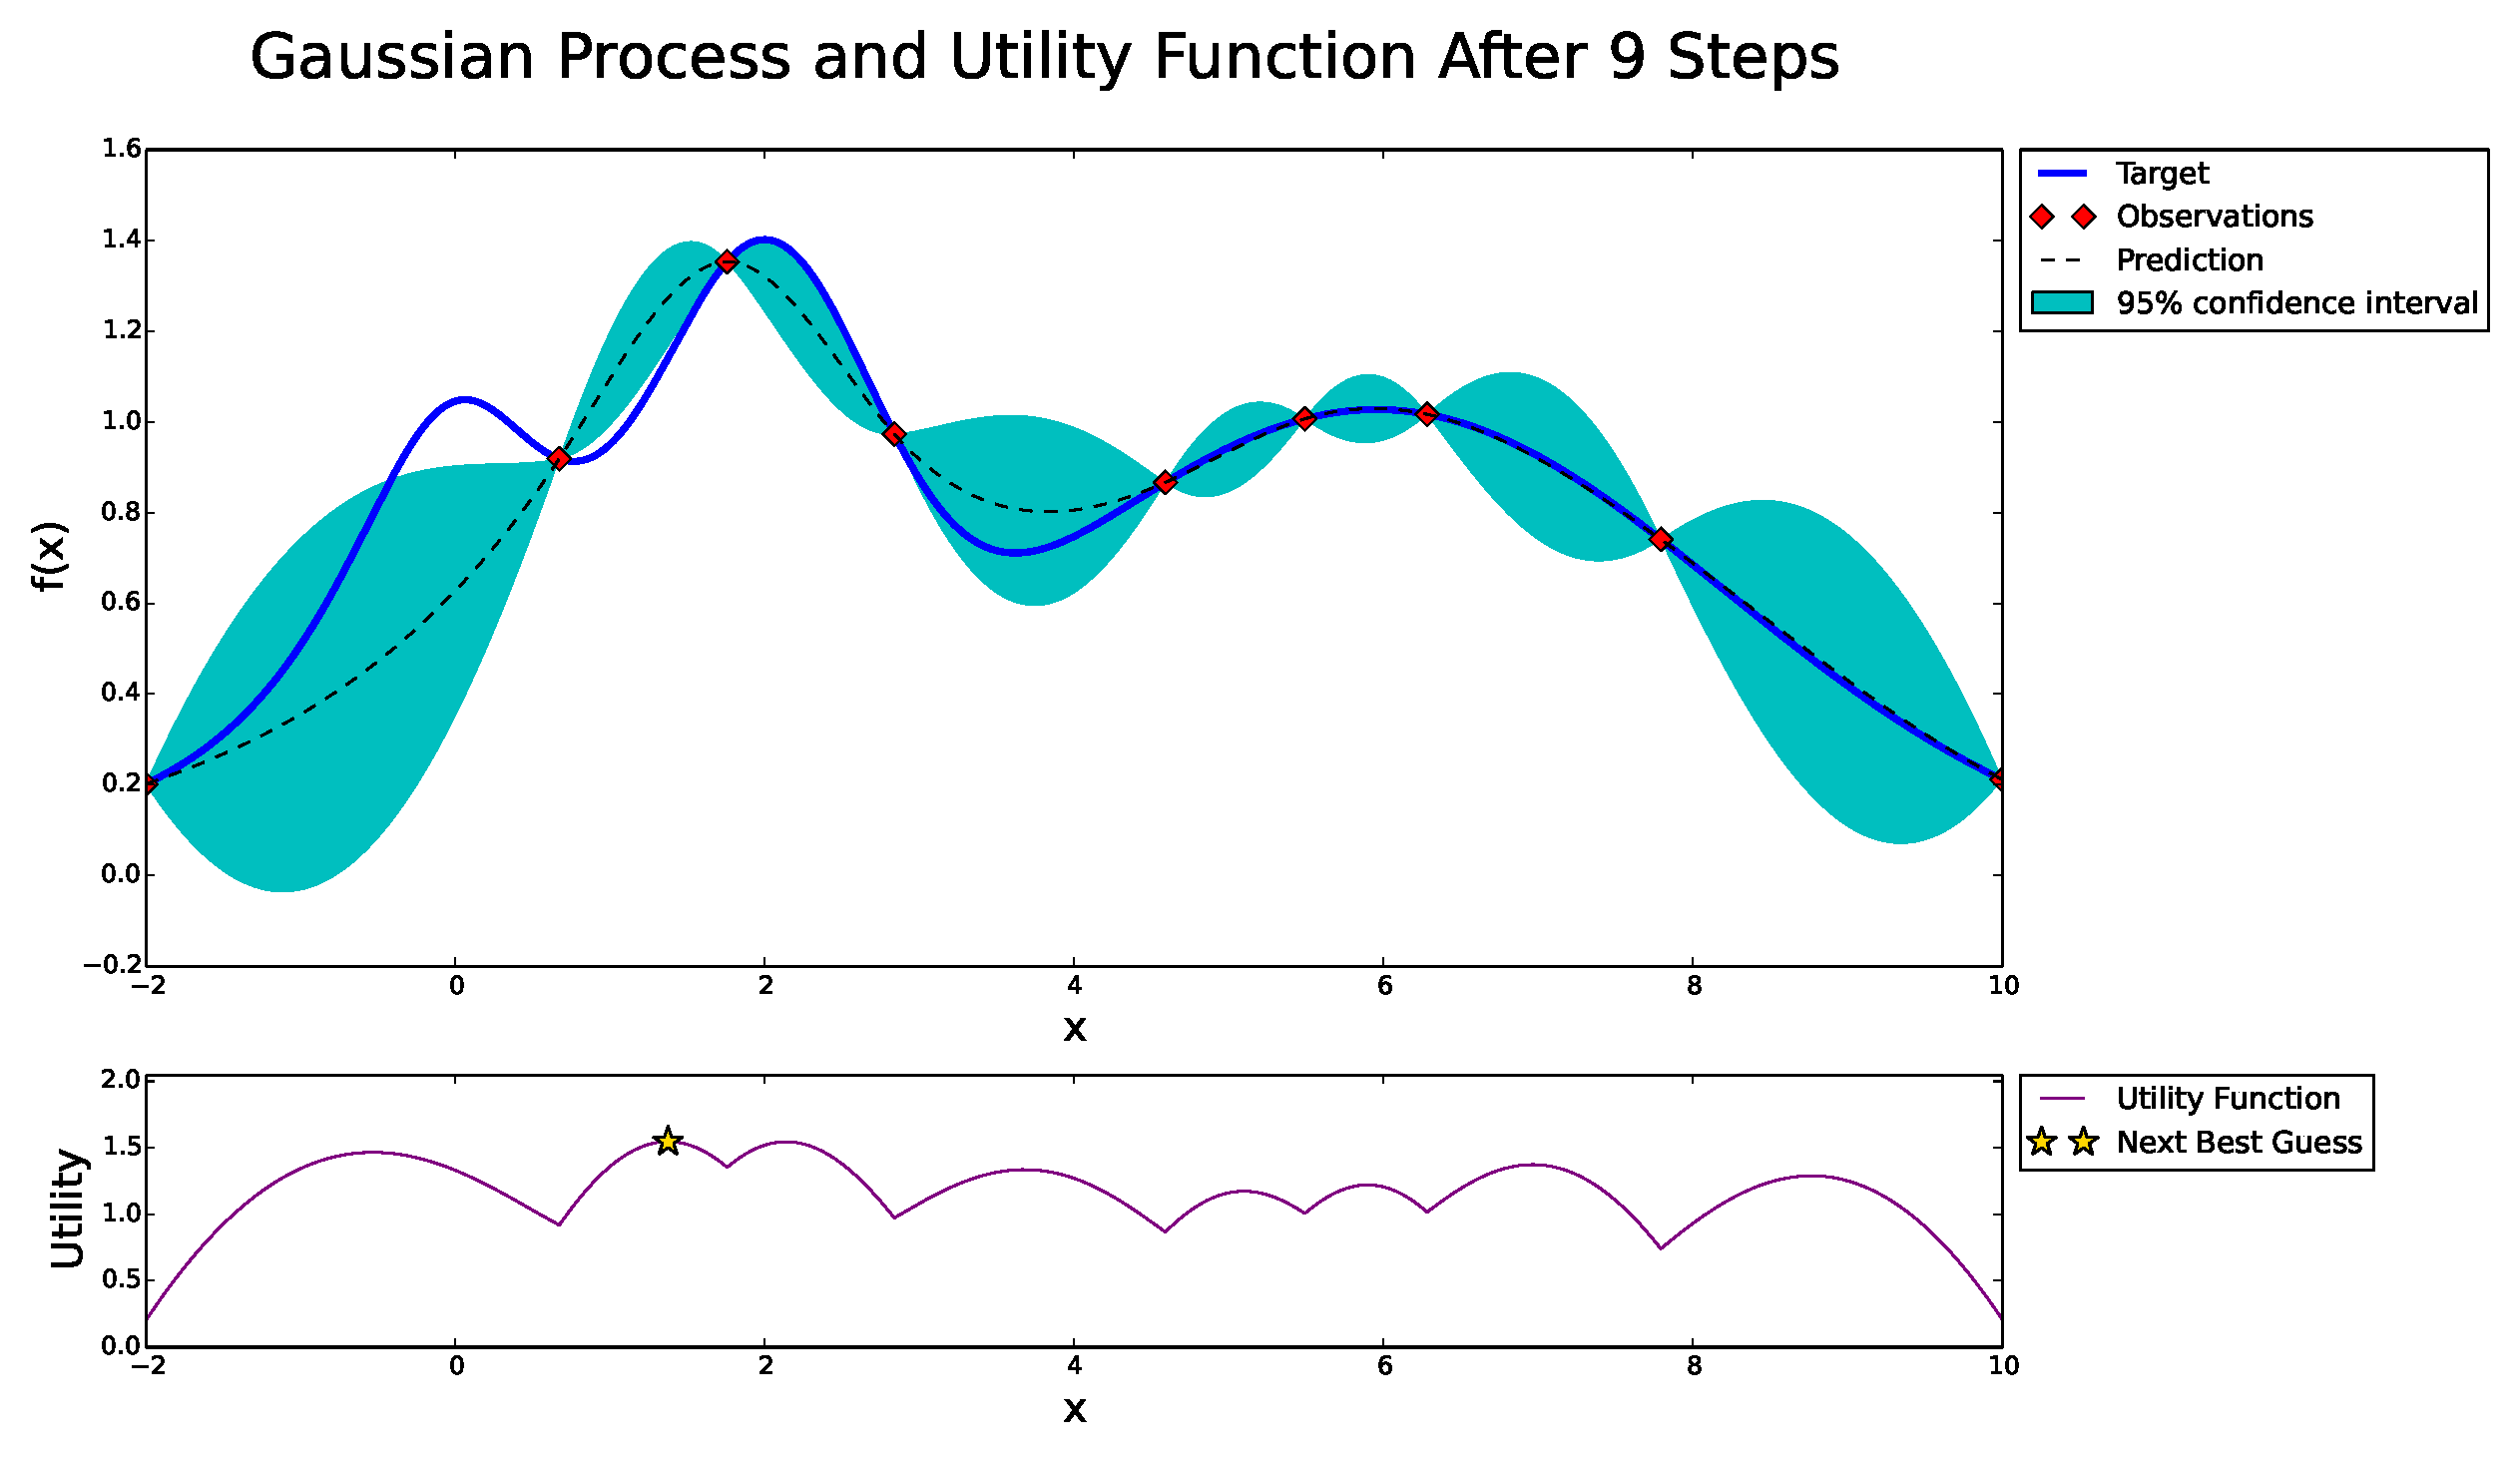
\includegraphics[width=0.8\textwidth]{figures/bayesian-optimization/fig7}
	
\end{frame}

\section{Demo \& Next Steps}

\begin{frame}
\frametitle{Implementation of Model-Optimization Routine}

\begin{itemize}
	\item<1-> \textbf{Exploration:} 'Randomly' navigating, writing execution trace to files
	\item<2-> \textbf{Optimization:} Objective function defined by performance in simulations:
	\begin{itemize}
		\item Goal area(s) reached (before time-out)?
		\item Time passed
		\item Part of goal area covered by corresponding final states
	\end{itemize}
	\vfill
	\item<3-> \textbf{Software:} Python, ROS, Morse simulator
	\item<3-> \textbf{Robot:} Scitos A5, mobile service robot
\end{itemize}

\end{frame}

\begin{frame}
\begin{center}

\Huge
\textbf{\textcolor{tudblue}{DEMO}}

\end{center}
\end{frame}

\begin{frame}
\frametitle{Next Steps}

\begin{itemize}
	\item<1-> Cost-Sensitive Optimization 
	\begin{itemize}
		\item BO acquisition based on \textit{Expected Improvement per second}
	\end{itemize}
	\item<2-> Identification of incomplete exploration data
	\begin{itemize}
		\item Feedback from simulation trajectories
		\item Use feedback in BO to reduce noise/uncertainty in observations
	\end{itemize}
	\item<3-> Variable Resolution in State-Space Acquisition
	\item<4-> Inspect influence of other variables in the optimization loop
	\begin{itemize}
		\item Discount factor $\gamma$ in MDP solver
		\item ML-algorithm (K-Means, GMM, $\ldots$)
		\item Gaussian-Process hyper-parameters?
	\end{itemize}
\end{itemize}
\end{frame}

\section{} % On purpose empty!

\begingroup
\setbeamertemplate{headline}{%
\leavevmode%
  \hbox{%
    \begin{beamercolorbox}[wd=\paperwidth,ht=2.5ex,dp=1.25ex]{palette tertiary}%
    \end{beamercolorbox}%
  }
}

% Title Sheet
\frame{\titlepage}

\begin{frame}[allowframebreaks]
\frametitle{References}\nocite{*}
\scriptsize
\bibliography{references}
\end{frame}

\endgroup

\bibliographystyle{abbrv}

\end{document}


